\documentclass[12pt, a4paper]{report}
\usepackage{graphicx} %LaTeX package to import graphics
\usepackage[shortlabels]{enumitem}
\usepackage{geometry}
\usepackage{xcolor}
\geometry{lmargin=30mm}
\usepackage[export]{adjustbox}
\usepackage{titlesec}
\usepackage{float}
\usepackage{listings}

\usepackage{hyperref}

\titleformat{\chapter}{\normalfont\huge}{\thechapter}{20pt}{\huge\bf}
\graphicspath{{images/}} %configuring the graphicx package
\title{Practica 4}
\author{Javier Izquierdo Hernández}
\date{\today}
\begin{document}
	\begin{titlepage}
		\centering
		{
\includegraphics[width=0.3\textwidth]{logo}\par}
		\vspace{1cm}
		{\bfseries\LARGE Universidad Rey Juan Carlos \par}
		\vspace{1cm}
		{\scshape\Large E.T.S. Ingeniería de Telecomunicación \par}
		\vspace{3cm}
		{\scshape\Huge Redes de Ordenadores para Robots y Máquinas Inteligentes \par}
		\vspace{3cm}
		{\itshape\Large Práctica 4\par}
		\vfill
		{\Large Autor: \par}
		{\Large Javier Izquierdo Hernández \par}
		\vfill
		{\Large \today \par}
	\end{titlepage}

\newpage
\renewcommand{\contentsname}{Contenidos}
\tableofcontents
\newpage

Descarga tu escenario de red para esta práctica del siguiente enlace:

\begin{center}
https://mobiquo.gsyc.urjc.es/practicas/ror/p4.html
\end{center}

Descomprime el fichero que contiene el escenario de NetGUI lab-tc.tgz.

\begin{figure}[h]
	\centering
	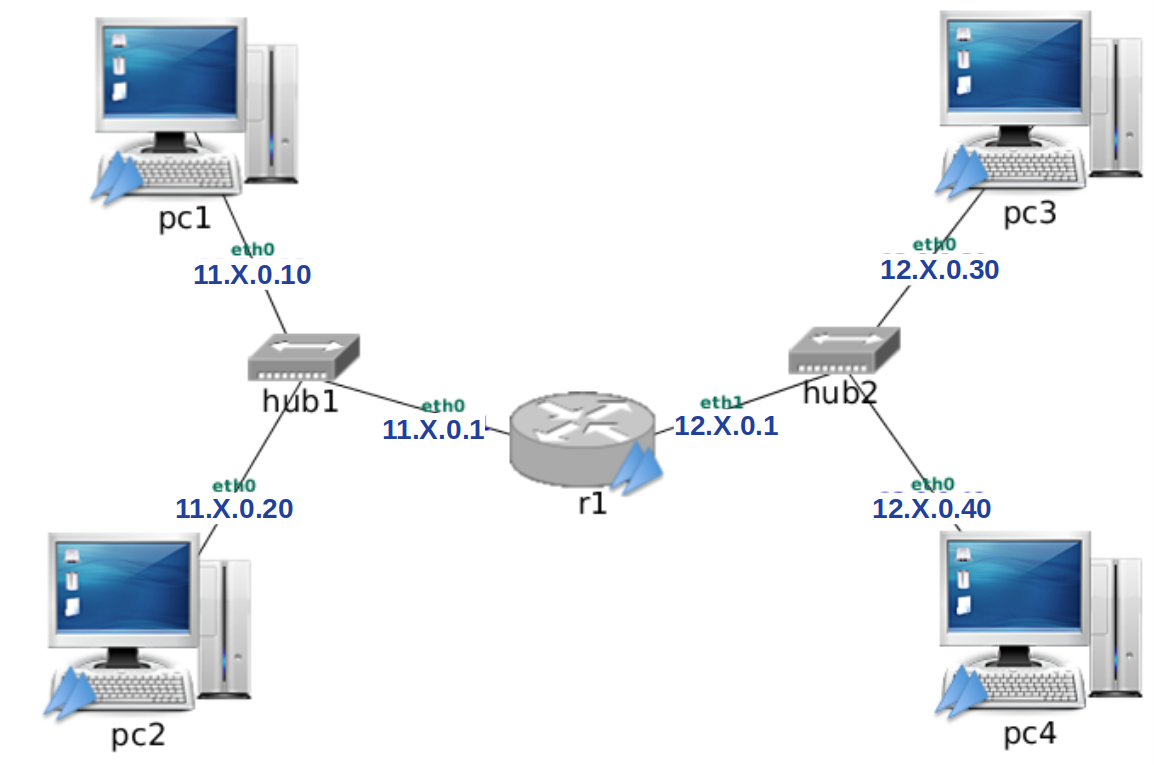
\includegraphics[width=0.8\textwidth]{enunciado1}
	\caption{Escenario para control de tráfico}
\end{figure}

\chapter{Control de Tráfico}
\section{Sin control de tráfico ni a la entrada ni a la salida}
El router r1 no tiene activado el control de tráfico en ninguna de sus interfaces.
\subsection{Un flujo de datos}
Inicia una captura en la interfaz r1(eth1) guardando el contenido en \textcolor{blue}{tc-01.cap}.\\

Arranca iperf en modo servidor UDP en pc3 y arranca iperf en modo cliente UDP en pc1 para
que envíe tráfico a 3M durante 10 segundos a pc3.\\

Observa en el servidor el informe que aparece al terminar de recibir el tráfico pc1 → pc3.
Carga la captura en wireshark y muestra el flujo de forma gráfica, incluye una imagen en la
memoria.
\begin{figure}[h]
	\centering
	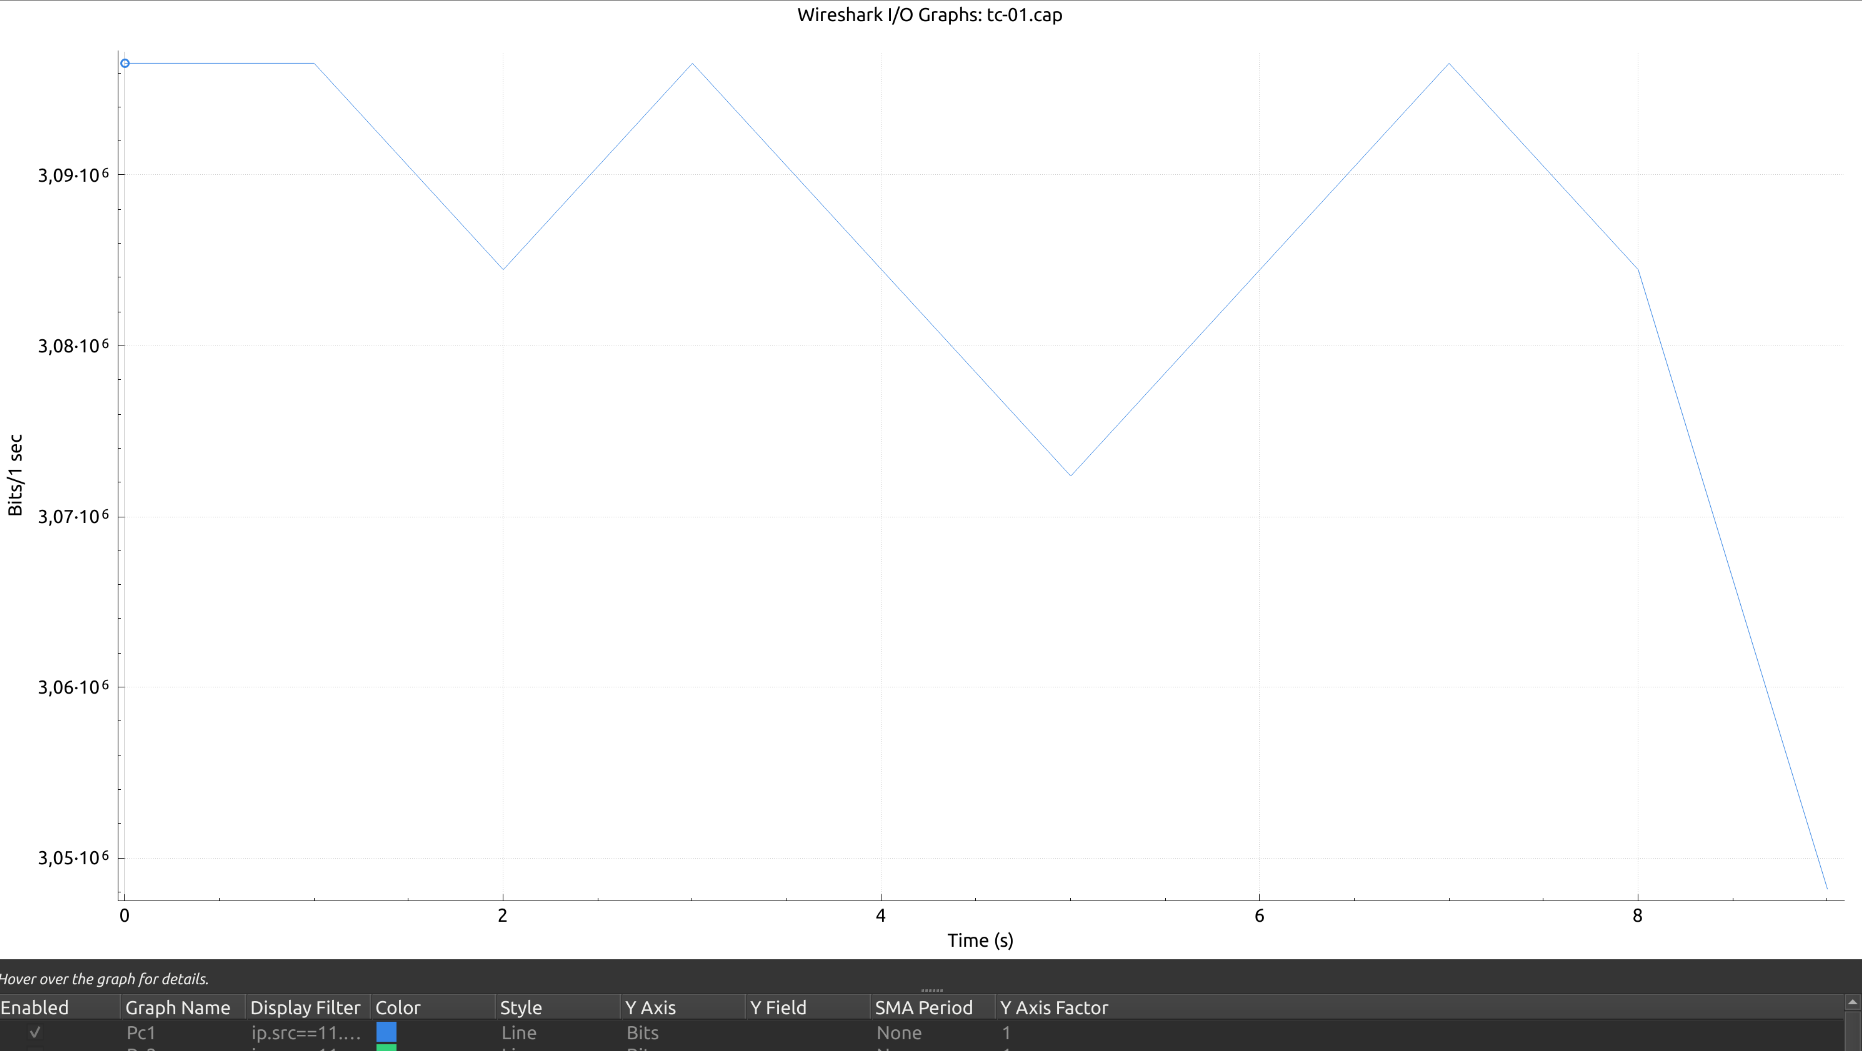
\includegraphics[width=0.8\textwidth]{ej1.1.1}
\end{figure}
\subsection{Dos flujos de datos}
\begin{itemize}
	\item Arranca iperf en modo servidor UDP en pc4.
	\item Arranca otro iperf en modo servidor UDP en pc3.
	\item Inicia una captura de tráfico en la interfaz eth1 de r1 (\textcolor{blue}{tc-02.cap}).
	\item Escribe (todavía sin ejecutar) el comando que arranca iperf en modo cliente UDP en pc1 para
	que envíe 3M al servidor pc3 en el sentido pc1 → pc3 durante 10 segundos.
	\item Escribe (todavía sin ejecutar) el comando que arranca iperf en modo cliente UDP en pc2 para
	que envíe 3M al servidor pc4 en el sentido pc2 → pc4 durante 10 segundos.
	\item Ejecuta los dos comandos anteriores uno a continuación de otro (lo más rápidamente que puedas)
	para que su ejecución se realice de forma simultánea.
	\item Interrumpe la captura una vez que los clientes hayan terminado de ejecutar iperf.
\end{itemize}
A continuación analiza los resultados obtenidos:
\begin{enumerate}
	\item Explica las estadísticas que muestran los servidores.\\
	
	Como esta puesta la política de cola por defecto, ambos servidores reciben la misma cantidad de datos que envían los clientes.
	\begin{figure}[h]
		\centering
		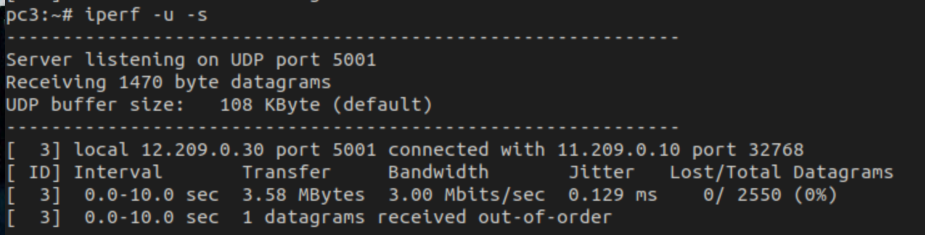
\includegraphics[width=0.8\textwidth]{ej1.1.2_1_a}\\
		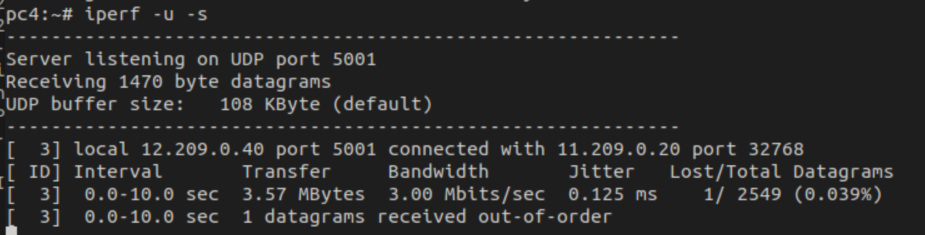
\includegraphics[width=0.8\textwidth]{ej1.1.2_1_b}\\
	\end{figure}
	\item Carga la captura en wireshark y muestra cada uno de los flujos de forma gráfica. Incluye una
	imagen en la memoria que muestre los flujos de forma gráfica. Explica el ancho de banda medido
	para cada uno de los flujos.\\
	\begin{figure}[H]
		\centering
		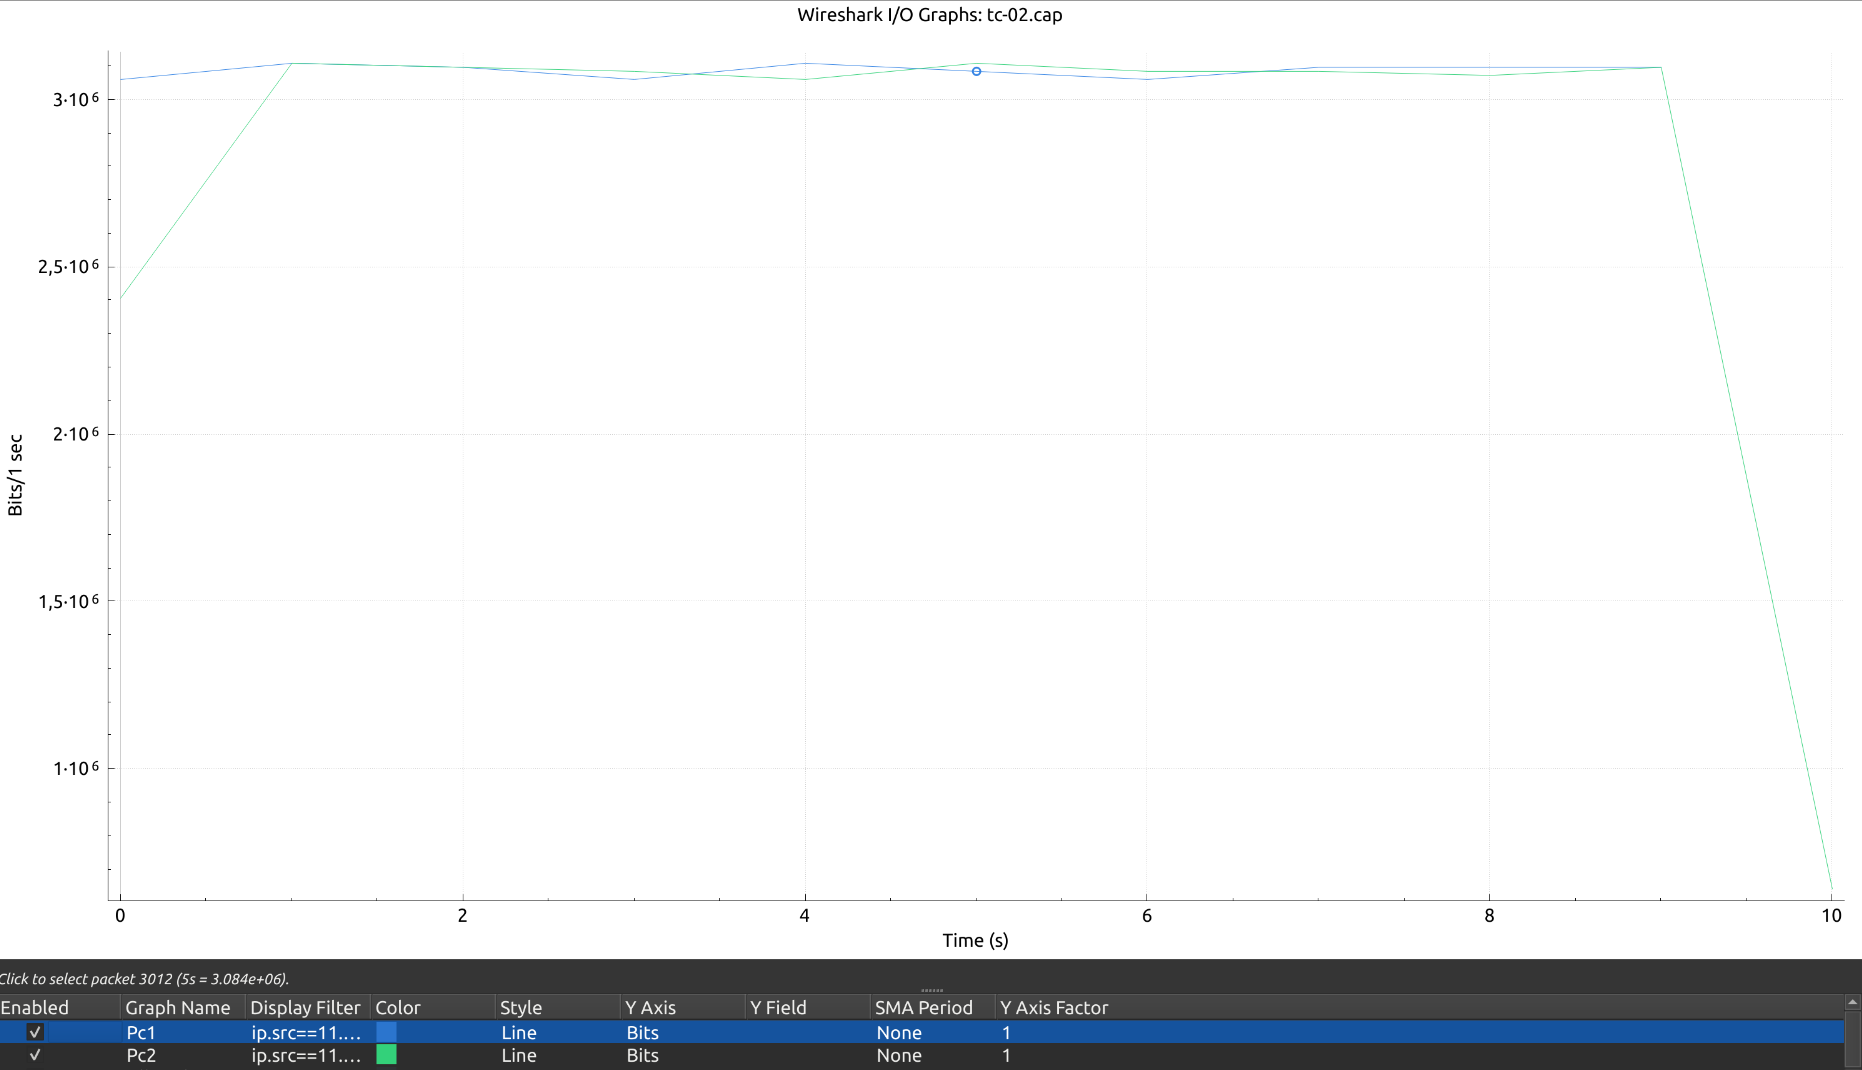
\includegraphics[width=0.8\textwidth]{ej1.1.2_2}
	\end{figure}
	El ancho de banda será de 3 M/s porque es la cantidad que hemos indicado y como se usa la política de cola por defecto, los datagramas pasan sin problema alguno.
\end{enumerate}
\section{Control de admisión para el tráfico de entrada}
Vamos a configurar r1 para restringir el tráfico de entrada distinguiendo 2 flujos de datos:
\begin{itemize}
	\item Flujo 1: origen pc1, se quiere restringir con TBF a una velocidad de 1 mbit y una cubeta de
	10k bytes.
	\item Flujo 2: origen pc2 se va a restringir a una velocidad de 2 mbit y una cubeta de 10k bytes.
\end{itemize}
Utiliza tc para definir esta configuración en la interfaz eth0 de r1, que es la interfaz de entrada
para los flujos 1 y 2. Haz que se aplique primero el filtro del flujo número 1 y después el del número
2. Guarda esta configuración en un fichero de script con el nombre \textcolor{blue}{tc-ingress.sh}:
\begin{center}
	\begin{verbatim}
		#!/bin/sh
		
		# Esto es un comentario
		echo "Borrando la disciplina de cola ingress en la interfaz eth0"
		
		tc qdisc del ...
		echo "Creando la disciplina de cola ingress en la interfaz eth0"
		tc qdisc add ...
		...
	\end{verbatim}
\end{center}
Una vez creado el script recuerda darle permisos de ejecución.\\

Si prefieres, puedes editar el script en la máquina real (Ubuntu) con un editor gráfico y luego
ejecutarlo.\\

IMPORTANTE: Escribe el script de forma que sólo borre la disciplina de cola si está definida, para
que no dé un error. Para ello, utiliza el comando \textcolor{blue}{tc qdisc show dev eth0} y comprueba su salida.
Si no devuelve nada, es que no hay ninguna qdisc definida, si devuelve algo es que hay una definida y
conviene borrarla primero antes de añadirla.\\

Incluye dentro de la memoria el contenido del script, así como de los scripts que desarrolles en los
siguientes apartados.\\

 Ver \ref{tc-ingress}, \ref{tc-egress-tbh}, \ref{tc-egress-tbh-prio} y \ref{tc-egress-htb}.

\begin{enumerate}
	\item Consulta la configuración actual de las disciplinas de cola configuradas por defecto en r1. Indica
	qué resultado has obtenido para cada una de las colas.
	\begin{figure}[H]
		\centering
		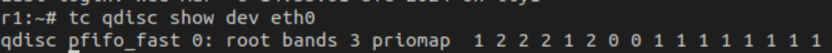
\includegraphics[width=0.8\textwidth]{ej1.2_1_a}
		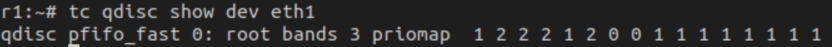
\includegraphics[width=0.8\textwidth]{ej1.2_1_b}
	\end{figure}
	He obtenido el mismo resultado para ambas, una priomap, que es la cola que viene por defecto.
	\item Realiza una prueba de tráfico como la del apartado anterior:
	\begin{itemize}
		\item Inicia una captura de tráfico en la interfaz eth1 de r1 (\textcolor{blue}{tc-03.cap})
		\item Arranca dos clientes y 2 servidores tal y como lo hiciste en el apartado 1.1.2.
		\item Interrumpe las capturas cuando los servidores hayan terminado de recibir todo el tráfico.
	\end{itemize}
	\item Explica las estadísticas que muestran los servidores.\\
	Como se limita el flujo de pc1 a pc3 a 1 mbit/s, se deben perder $2/3$ de los 3 mbit/s que manda pc1 como se ve en la imagen inferior.
	\begin{figure}[H]
		\centering
		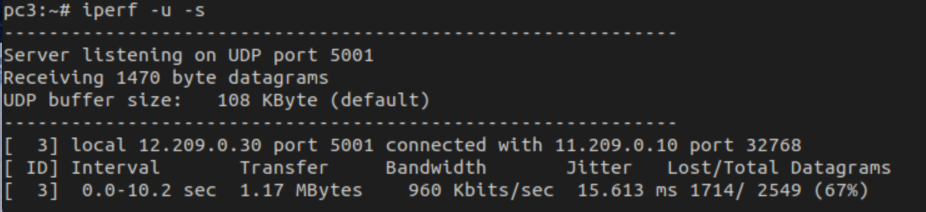
\includegraphics[width=0.8\textwidth]{ej1.2_3_a}
	\end{figure}	
	Como se limita el flujo de pc2 a pc4 a 2 mbit/s, se deben perder $1/3$ de los 3 mbit/s que manda pc1 como se ve en la imagen inferior.
	\begin{figure}[H]
		\centering
		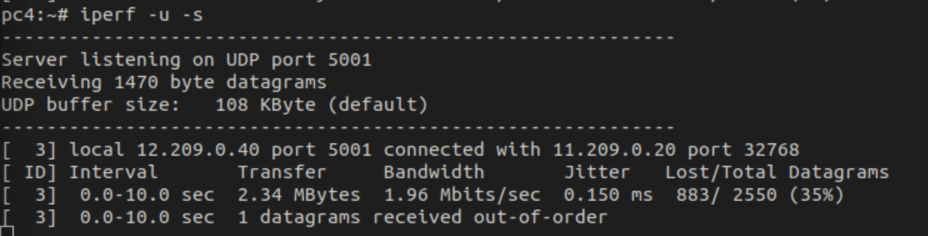
\includegraphics[width=0.8\textwidth]{ej1.2_3_b}
	\end{figure}
 	\item Carga las capturas en wireshark y muestra cada uno de los flujos de forma gráfica. Incluye una
	imagen en la memoria que muestre los flujos de ambas capturas de forma gráfica. Explica el
	ancho de banda medido para cada uno de los flujos.
	\begin{figure}[H]
		\centering
		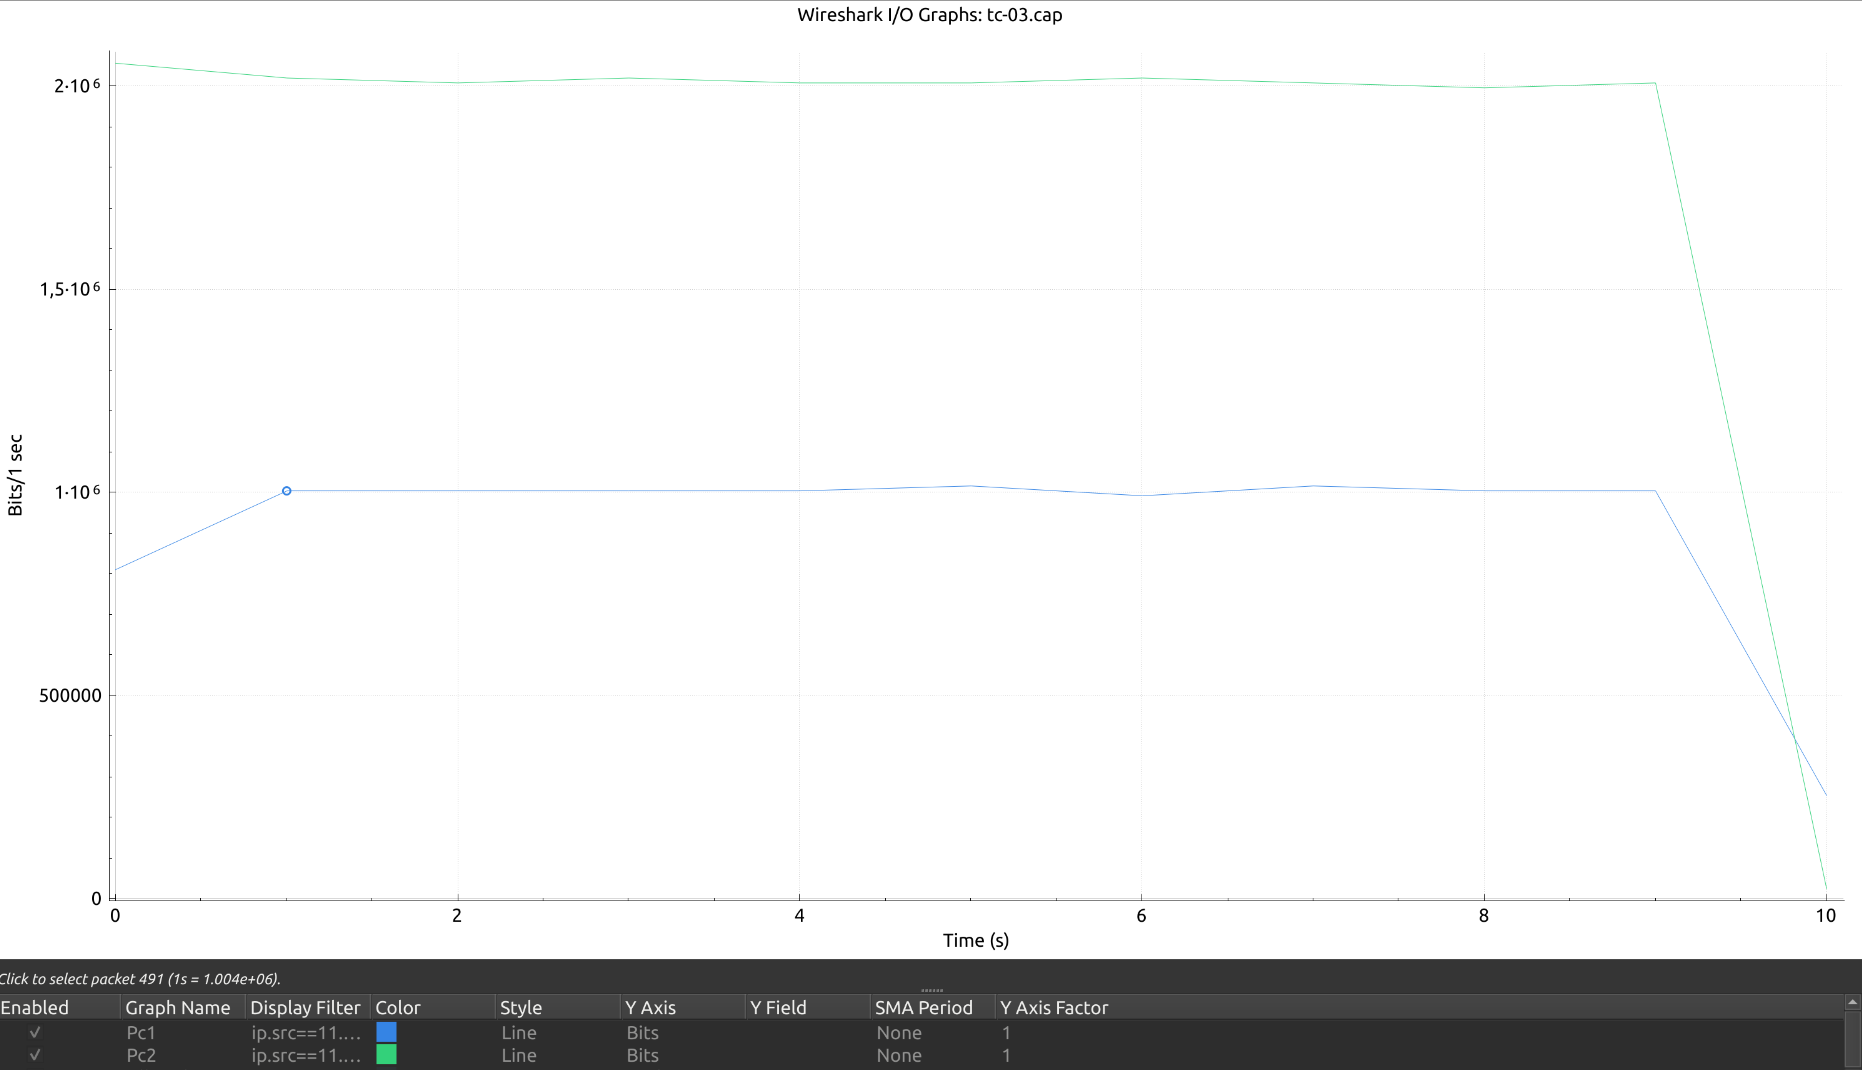
\includegraphics[width=0.8\textwidth]{ej1.2_4}
	\end{figure}
	Como he explicado en el apartado anterior y como se puede ver en la captura, el flujo de datos que manda pc1 se capa a 1 mbit/s, mientras que el de pc2 se capa a 2 mbit/s. Y el resto del tráfico se descarta. 
	\item Consulta la configuración actual de las disciplina de cola configurada a la entrada en eth0. Indica
	el número de paquetes recibidos y el número de paquetes descartados.\\
	
	La configuración de la cola configurada en eth0, es la que hemos puesto en el script, aunque sigue siendo una priomap.
	\begin{figure}[H]
		\centering
		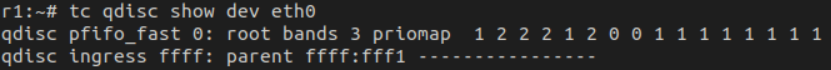
\includegraphics[width=0.8\textwidth]{ej1.2_5}
	\end{figure}
	Como se puede ver en las imágenes del apartado 3, pc3 recibe 835 y descarta 1714 de un total de 2549, lo que hace un total de un 33\% de datagramas recibidos. En cuanto a pc4, este recibe 1667 y descarta 883 de un total de 2549, lo que hace un total de un 65\% de datagramas recibidos. 
\end{enumerate}
\section{Disciplinas de colas para el tráfico de salida}
\subsection{Token Bucket Filter (TBF)}
Mantén la configuración del tráfico de entrada en r1 que has realizado en el apartado anterior en
el script tc-ingress.sh.
\begin{itemize}
	\item Define en r1 para su interfaz eth1 una disciplina TBF de salida con tasa de envío de 1.5 mbit,
	tamaño de cubeta 10k y latencia 10 ms, y guarda la configuración en un nuevo script
	\textcolor{blue}{tc-egress-tbf.sh}.
	\item Inicia una captura de tráfico en la interfaz eth1 de r1 (\textcolor{blue}{tc-04.cap}).
	\item Arranca 2 clientes y 2 servidores tal y como lo hiciste en el apartado 1.1.2.
	\item Interrumpe la captura cuando los servidores hayan terminado de recibir todo el tráfico.
\end{itemize}
A continuación analiza los resultados obtenidos:
\begin{enumerate}
	\item Explica las estadísticas que muestran los servidores.\\
	
	Como se limita el flujo de pc1 a 1 mbit/s y el de pc2 a 2 mbit/s, se puede ver que pc4 deberá recibir el doble que pc3 aproximadamente. Pero como ahora en r1, se limita la salida a 1.5 mbit, en vez de los 3 mbit/s del apartado anterior se reducirá el flujo de salida a 1.5 mbit/s.
	\begin{figure}[H]
		\centering
		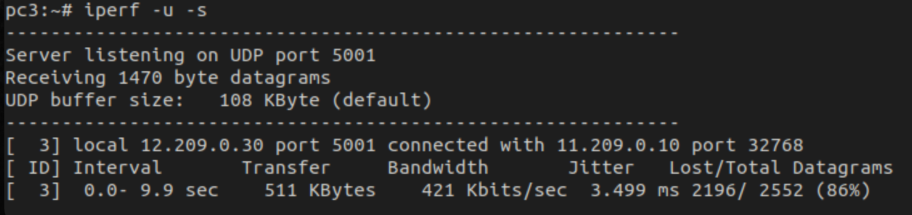
\includegraphics[width=0.8\textwidth]{ej1.3.1_1_a}
		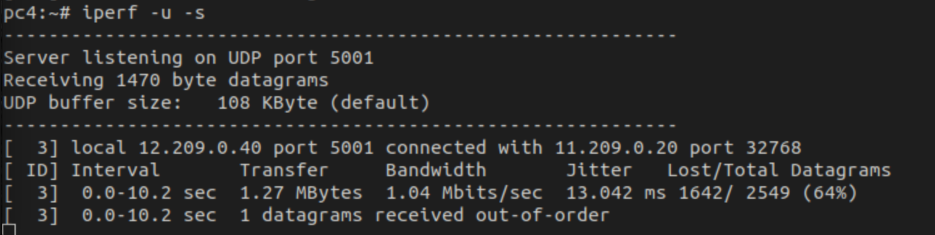
\includegraphics[width=0.8\textwidth]{ej1.3.1_1_b}
	\end{figure}
	\item Carga la captura en wireshark y muestra cada uno de los flujos de forma gráfica. Explica el
	ancho de banda medido para cada uno de los flujos.
	\begin{figure}[H]
		\centering
		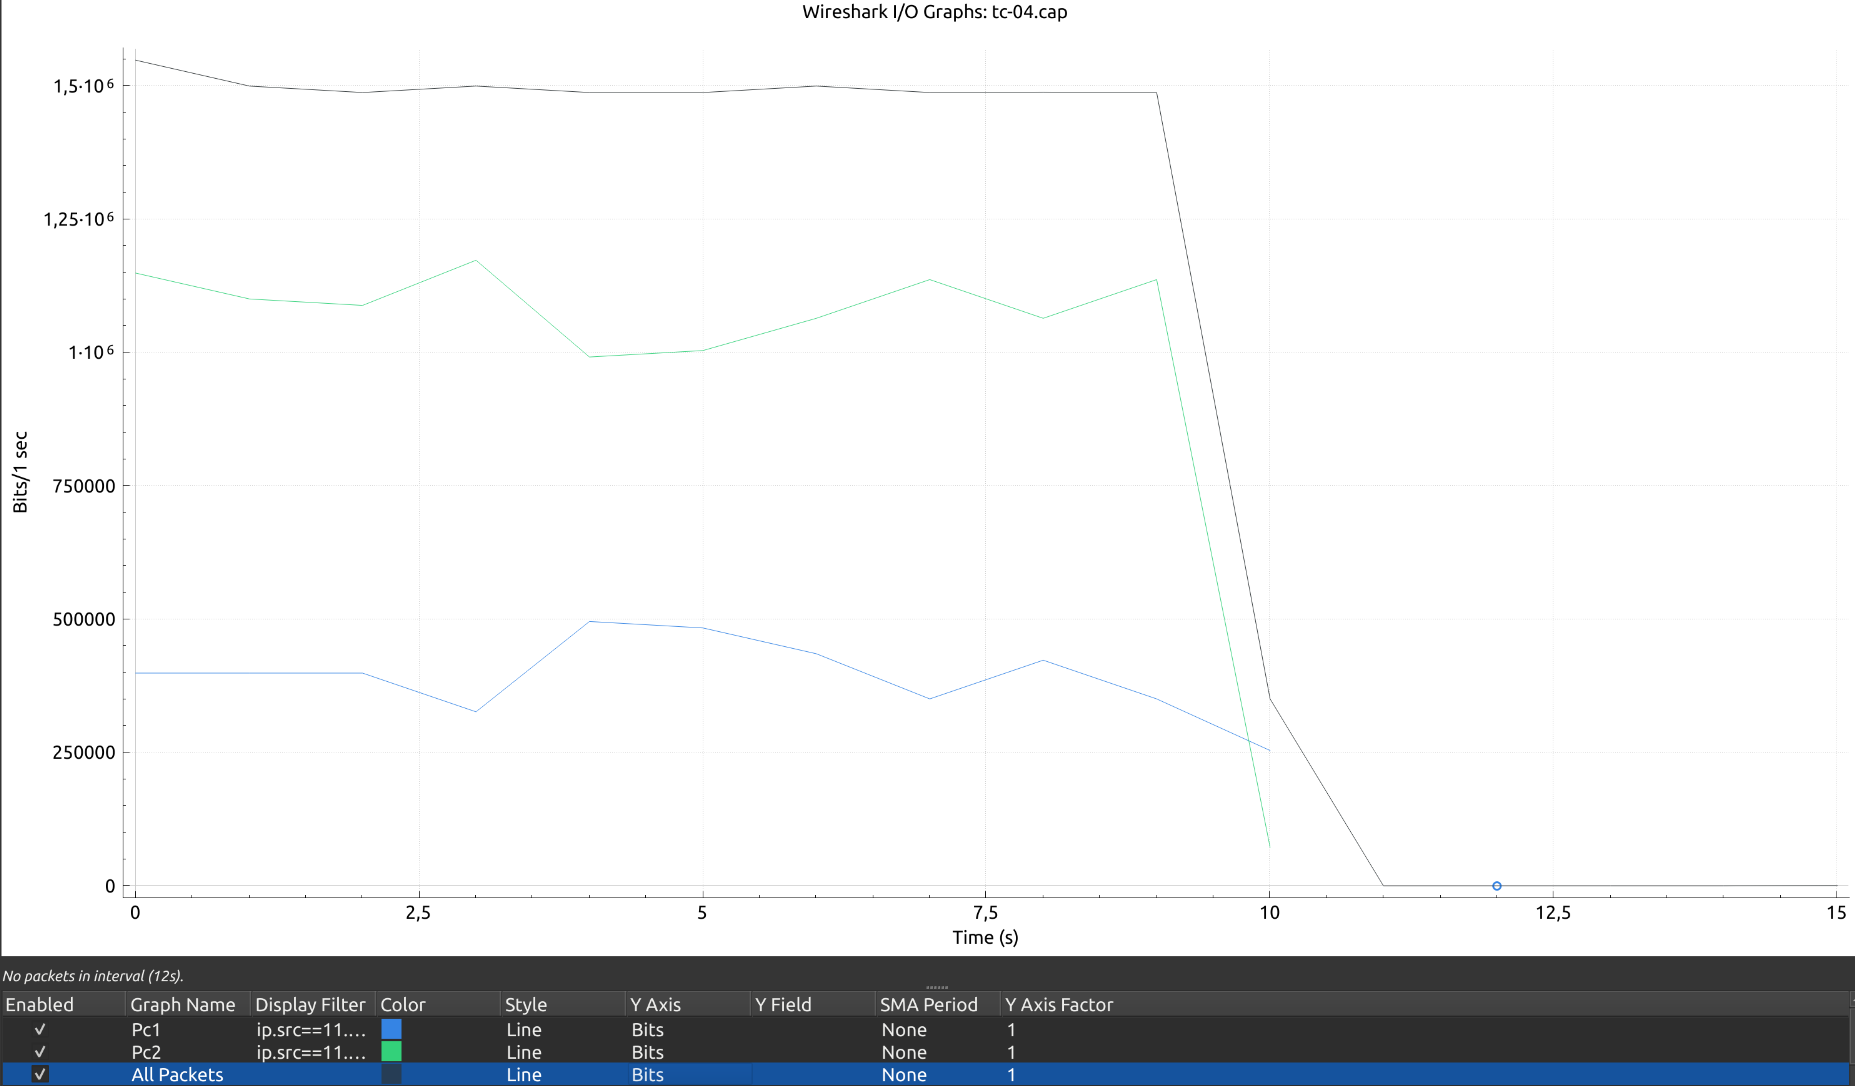
\includegraphics[width=0.8\textwidth]{ej1.3.1_2}
	\end{figure}
	Como he explicado en el apartado anterior y como se puede ver en la captura, el flujo de datos que manda pc1 oscila alrededor de 400-500 kbit/s, mientras que el de pc2 lo hace en torno a 1-1.2 mbit/s. También se puede ver que la suma de ambos flujos se mantiene estable en el tope 1.5 mbit/s, y que acaba con un poco de delay gracias a los 10 ms puestos. Al igual que anteriormente el resto de mensajes se descartan. 
\end{enumerate}
Modifica la configuración de TBF de salida para que ahora tenga una latencia de 20 segundos
(NOTA: ahora son 20 segundos en vez de 10 milisegundos) y realiza la misma prueba que antes 2 .
Llama ahora a la captura \textcolor{blue}{tc-05.cap}.\\

Interrumpe la captura cuando haya pasado tiempo suficiente para que termine de llegar todo el
tráfico a los servidores (será unos 20 segundos después de que comenzó a enviarse). A continuación
analiza los resultados obtenidos:
\begin{enumerate}
	\setcounter{enumi}{2}
	\item Explica las estadísticas que muestran los servidores.\\
	
	Las estadísticas se pueden explicar de la misma manera que en el apartado 1, con la excepción de que ahora en vez de ser el intervalo entre 0 y 10, ahora será de 0 a 20 segundos. También es importante recordar que estas cantidades de transferencia son las mismas que solo con el filtro en la entrada, pero con el ancho de banda reducido a la mitad, ya que el tiempo se dobla.
	\begin{figure}[H]
		\centering
		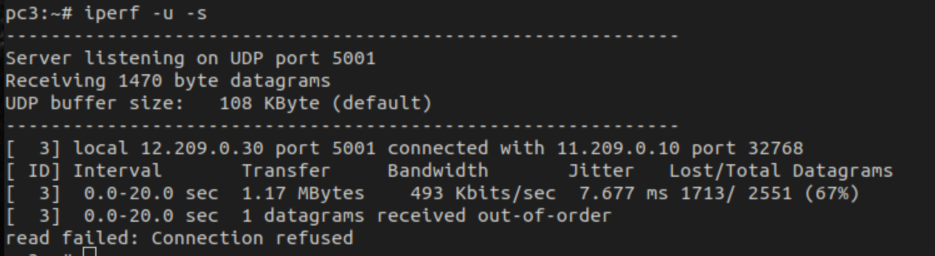
\includegraphics[width=0.8\textwidth]{ej1.3.1_3_a}
		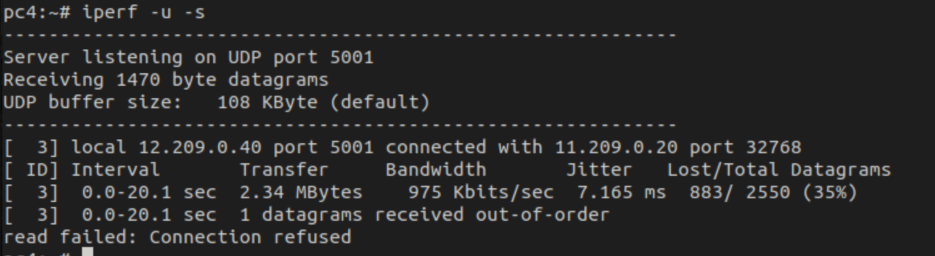
\includegraphics[width=0.8\textwidth]{ej1.3.1_3_b}
	\end{figure}
	\item Carga la captura en wireshark y muestra cada uno de los flujos de forma gráfica. Incluye una
	imagen en la memoria que muestre los flujos de forma gráfica. Explica el ancho de banda medido
	para cada uno de los flujos.
	\begin{figure}[H]
		\centering
		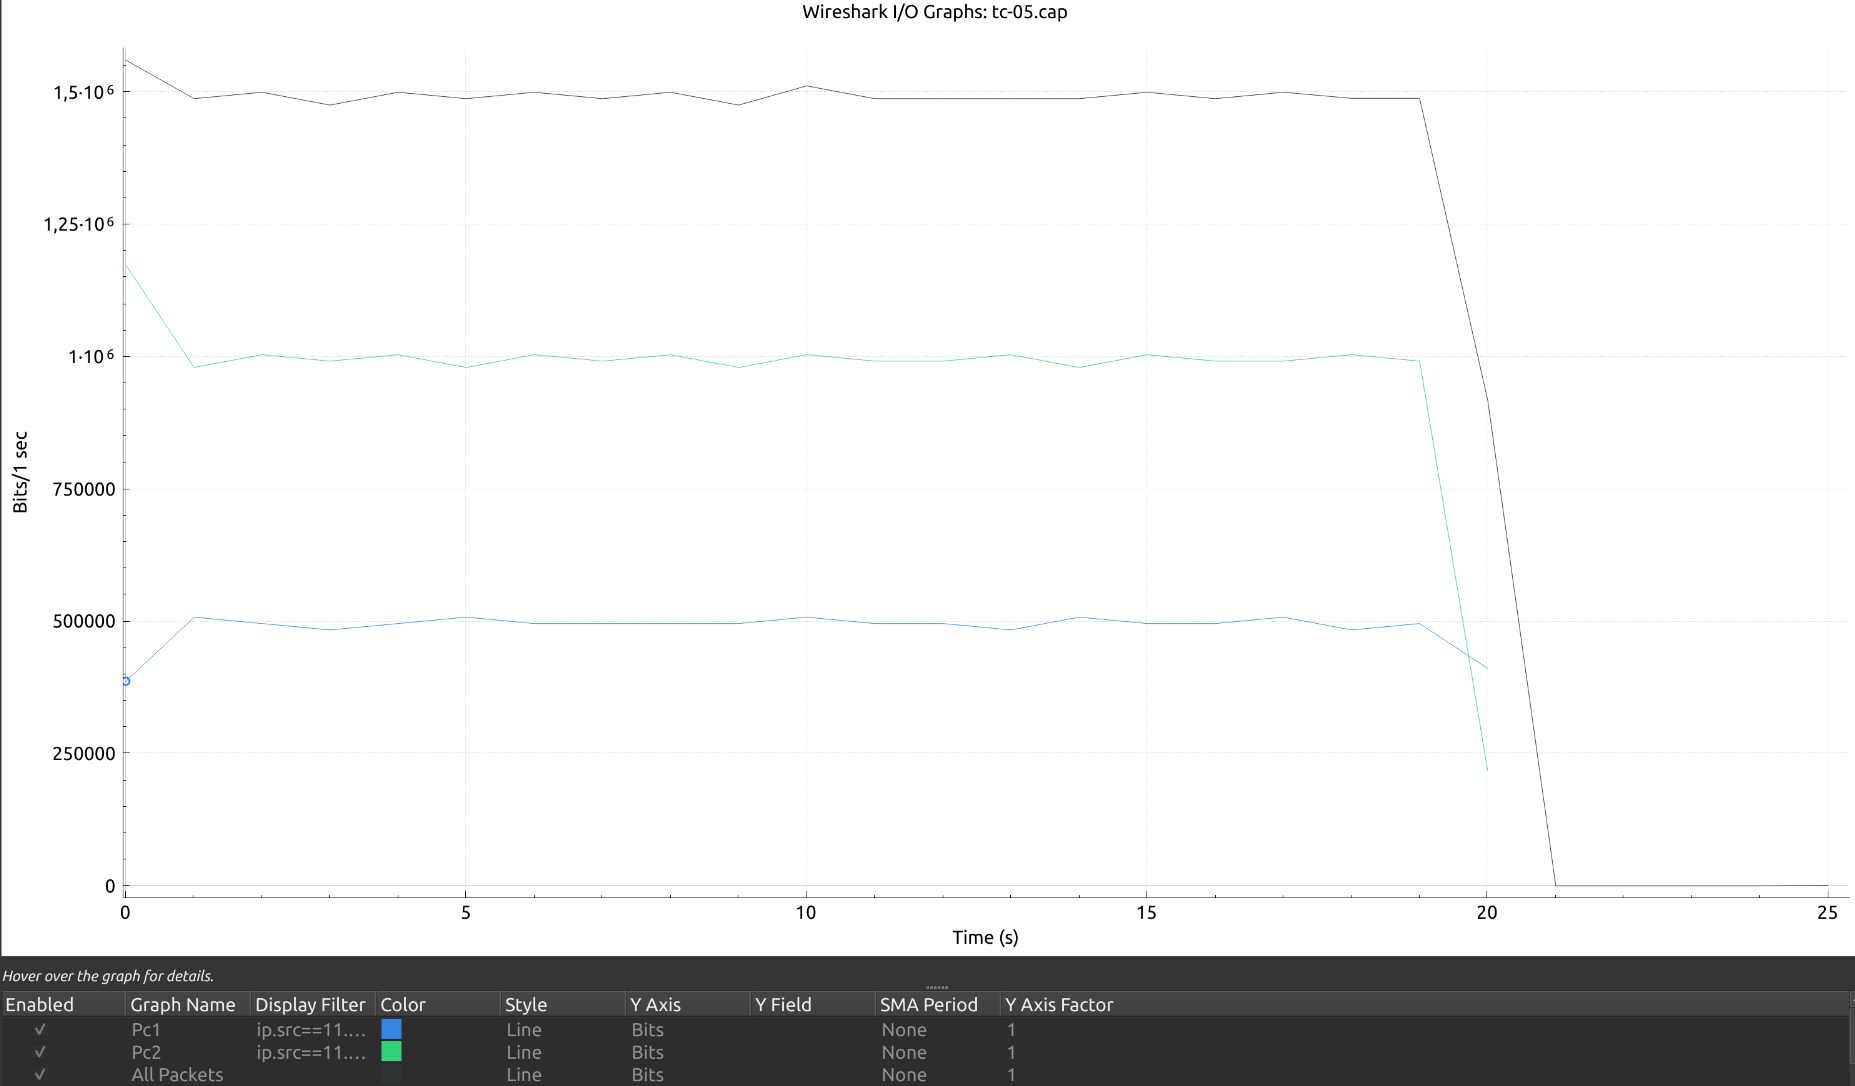
\includegraphics[width=0.8\textwidth]{ej1.3.1_4}
	\end{figure}
	Al igual que en el apartado 2, pero esta vez en vez de descartar el resto de paquetes justo después de que pasaran 10 ms, ahora se espera hasta los 20 segundos, que es cuando todo el tráfico que ha entrado a r1 es enviado.
	\item ¿Cuánto tiempo ha tardado r1 en realizar el reenvío de todo el tráfico? Relaciona este valor con
	la cantidad de datos que tenía que reenviar y la tasa de envío que estaba utilizando r1. Del
	tráfico originalmente enviado por pc1 y pc2, ¿cuánto ha sido descartado en la disciplina de cola
	asociada a eth0 de r1? ¿Y cuánto ha sido descartado en la disciplina asociada a eth1 de r1?\\
	
	R1 ha tardado 20 segundos en realizar el reenvío, que es el doble del tiempo durante el que envían pc1 y pc2, ya que el filtro de salida reduce la salida de 3 mbit/s a 1.5 mbit/s.\\
	
	Luego el tráfico de pc1 y pc2 solo ha sido descartado por la disciplina de la cola asociada con eth0, ya que se ha enviado el mismo tráfico que cuando solo estaba esta.
\end{enumerate}
\subsection{TBF + PRIO}
Mantén la configuración del tráfico de entrada en r1 que has realizado en el apartado anterior en
el script tc-ingress.sh. Borra la disciplina de cola de salida TBF configurada en la interfaz eth1 de
r1.\\

La configuración TBF en el apartado 1.3.1 permite gestionar la tasa de envío para que no supere
el valor configurado, en nuestro caso 1.5Mbit. Esta disciplina de cola es sin clases y trata a todos los
paquetes por igual. Ahora vamos a querer fijar la tasa de envío de r1 pero tratando los paquetes con
diferentes prioridades.\\

Toma como punto de partida esta configuración para que ahora se atienda el tráfico de salida según
diferentes prioridades, configurando una disciplina de cola con prioridad que sea hija de la disciplina
TBF.
\begin{itemize}
	\item Escribe un script en r1, \textcolor{blue}{tc-egress-tbf-prio.sh}, para configurar TBF con los siguientes
	parámetros: ancho de banda 1.5 mbit, cubeta 10k y latencia 20s. Crea una disciplina de cola hija con prioridad de tal forma que se asignen las siguientes prioridades:
	\begin{itemize}
		\item Prioridad 1 (más prioritario): tráfico de la dirección IP origen pc1
		\item Prioridad 2 (prioridad intermedia): tráfico de la dirección IP origen pc2
		\item Prioridad 3 (menos prioritario): sin definir, pues no lo necesitamos.
	\end{itemize}
	\item Inicia una captura de tráfico en la interfaz eth1 de r1 (\textcolor{blue}{tc-06.cap}).
	\item Arranca 2 clientes y 2 servidores tal y como lo hiciste en el apartado 1.1.2.
	\item Interrumpe la captura cuando haya pasado tiempo suficiente para que termine de llegar todo el
	tráfico a los servidores (será unos 20 segundos después de que comenzó a enviarse).
\end{itemize}
A continuación analiza los resultados obtenidos:
\begin{enumerate}
	\item Explica las estadísticas que muestran los servidores.\\
	
	Como pc1 tiene más prioridad acaba antes que pc2, y por lo tanto su ancho de banda será mayor que antes cuando no tenía prioridad.
	\begin{figure}[H]
		\centering
		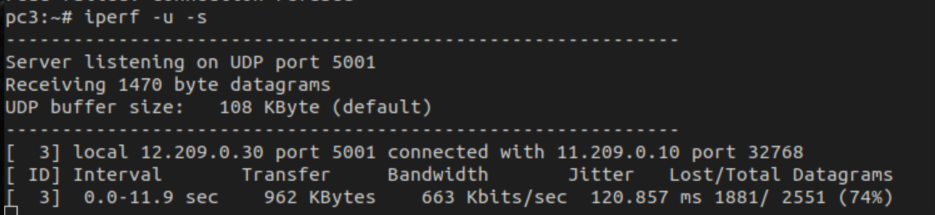
\includegraphics[width=0.8\textwidth]{ej1.3.2_1_a}
		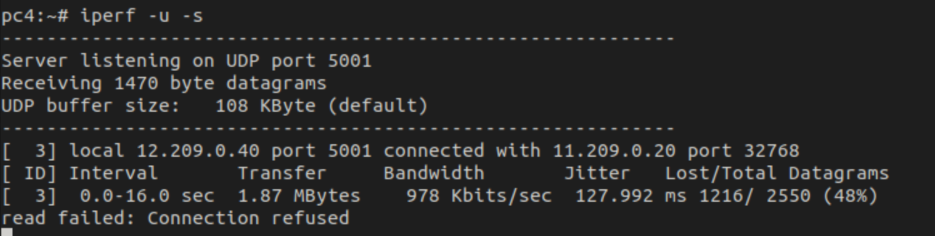
\includegraphics[width=0.8\textwidth]{ej1.3.2_1_b}
	\end{figure}
	\item Carga la captura en wireshark y muestra cada uno de los flujos de forma gráfica. Incluye una
	imagen en la memoria que muestre los flujos de forma gráfica. Explica la evolución en el tiempo
	del ancho de banda medido para cada uno de los flujos.
	\begin{figure}[H]
		\centering
		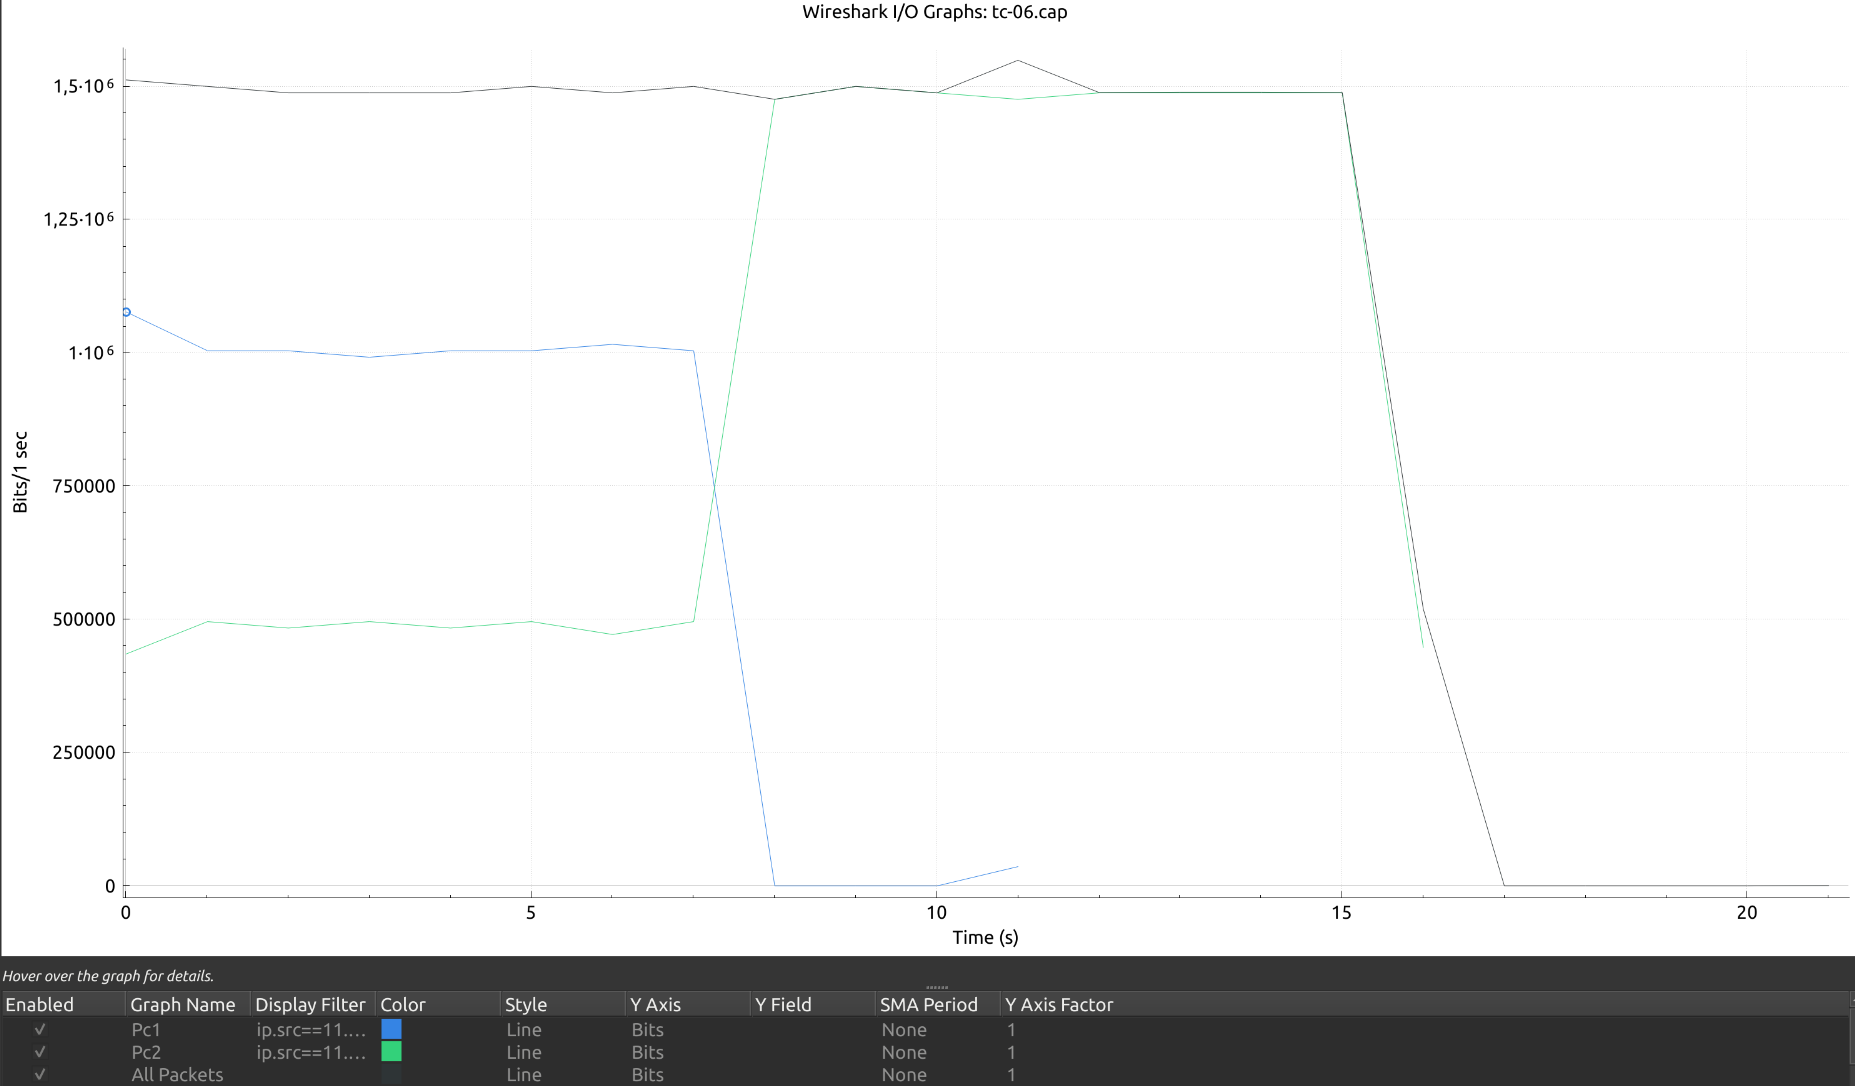
\includegraphics[width=0.8\textwidth]{ej1.3.2_2}
	\end{figure}
	Como el flujo desde pc1 tiene prioridad y esta capado en la entrada a 1 mbit/s, este será siempre 1 mientras que envíe mensajes, mientras que pc2 será 0.5 mbit/s (el resto) siempre que pc1 envíe el flujo de datos.\\
	Luego cuando pc1 no este, el flujo de datos desde pc2 se enviará ocupando todo el ancho de banda disponible, 1.5 mbit/s.
\end{enumerate}
\subsection{Hierarchical token Bucket (HTB)}
Mantén la configuración del tráfico de entrada en r1 que has realizado en el apartado anterior en
el script tc-ingress.sh. Borra la disciplina de cola de salida configurada en la interfaz eth1 de r1.
\begin{itemize}
	\item Escribe un script en r1, \textcolor{blue}{tc-egress-htb.sh}, para configurar en su interfaz eth1 una disciplina
	HTB de salida con ancho de banda 1.2 mbit. Reparte el ancho de banda de esta interfaz de
	salida de la siguiente forma:
	\begin{itemize}
		\item 700kbit para el tráfico con origen en pc1, ceil 700kbit.
		\item 500kbit para el tráfico con origen en pc2, ceil 500kbit.
	\end{itemize}
	\item Inicia una captura de tráfico en la interfaz eth1 de r1 (\textcolor{blue}{tc-07.cap}).
	\item Arranca 2 clientes y 2 servidores tal y como lo hiciste en el apartado 1.1.2.
	\item Interrumpe la captura cuando haya pasado tiempo suficiente para que termine de llegar todo el
	tráfico a los servidores (será unos 20 segundos después de que comenzó a enviarse). iperf.
\end{itemize}
A continuación analiza los resultados obtenidos:
\begin{enumerate}
	\item Explica las estadísticas que muestran los servidores.\\
	
	Como el flujo de pc1 se capa 700 kbit/s el ancho de banda será ese, mientras que la transferencia será de todos los datos que tenía que enviar. Y la duración del envío aumenta de 10 a 14.5 segundos.\\
	
	Algo similar ocurre con el flujo de pc2 pero con el ancho de banda siendo 500 kbit/s y el intervalo 34 segundos.
	\begin{figure}[H]
		\centering
		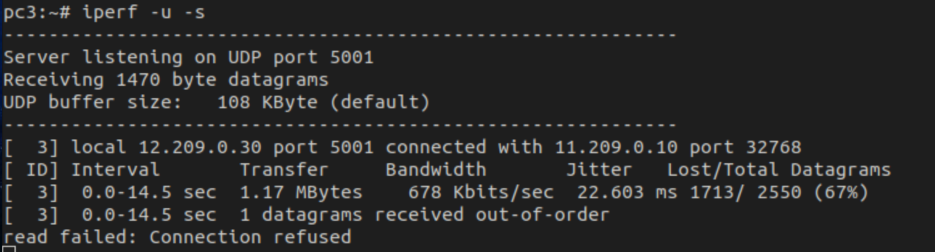
\includegraphics[width=0.8\textwidth]{ej1.3.3_1_a}
		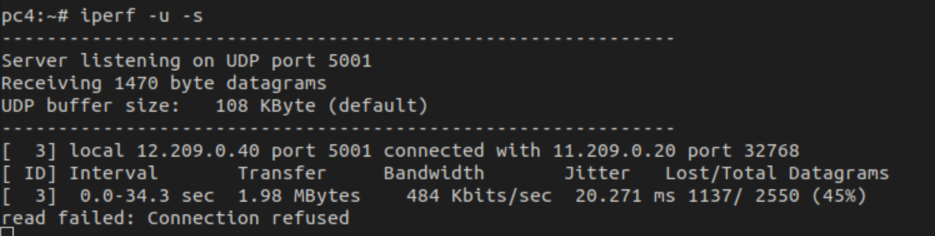
\includegraphics[width=0.8\textwidth]{ej1.3.3_1_b}
	\end{figure}
	\item Carga la captura en wireshark y muestra cada uno de los flujos de forma gráfica. Explica la
	evolución en el tiempo del ancho de banda medido para cada uno de los flujos.
	\begin{figure}[H]
		\centering
		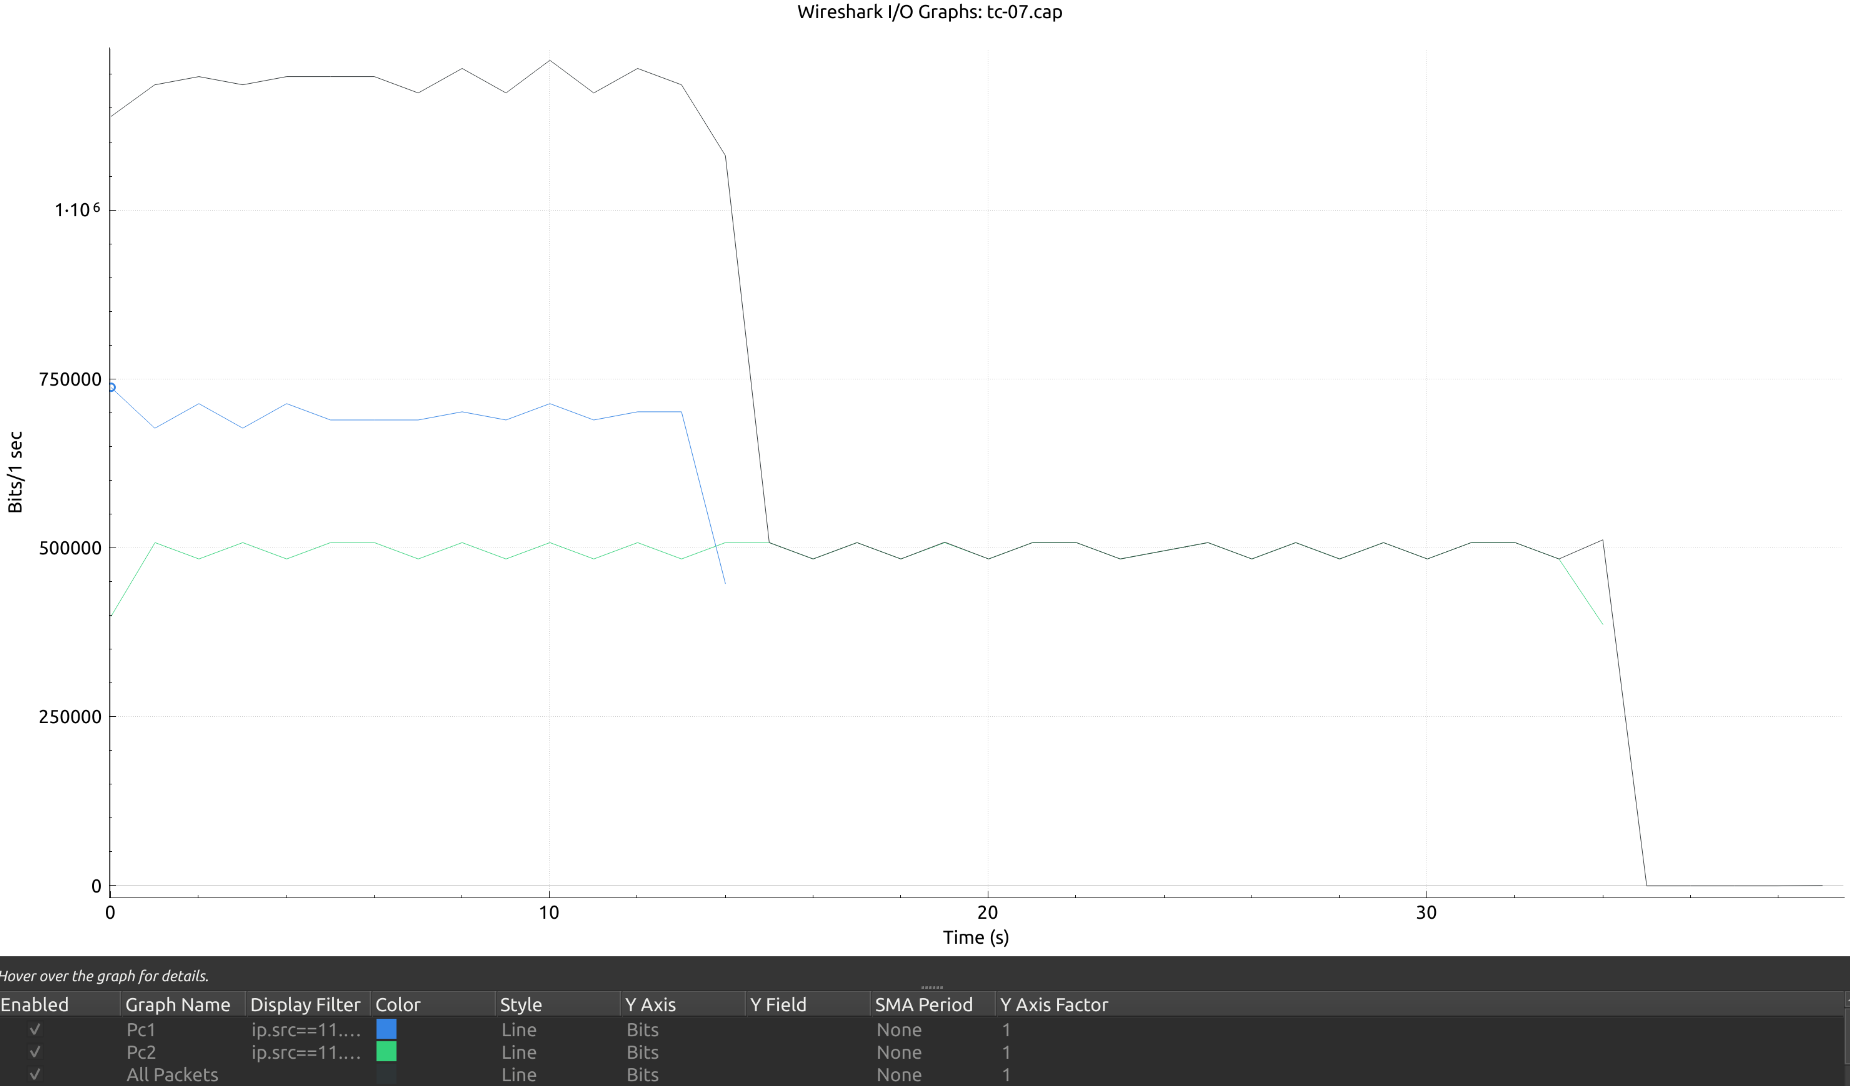
\includegraphics[width=0.8\textwidth]{ej1.3.3_2}
	\end{figure}
	Se ve que el flujo máximo que sale de r1 se mantiene estable en 1.2 mbit/s mientras que pc1 envia a 0.7 mbit/s y pc2 envía a 0.5 mbit/s. También se puede apreciar que r1 encola el tráfico hasta reenvirlo todo.
\end{enumerate}
Modifica la configuración de ceil en cada uno de los flujos para que puedan utilizar 1.2Mbit.
Realiza la misma prueba que antes capturando de nuevo el tráfico (\textcolor{blue}{tc-08.cap}) y analiza los resultados
obtenidos:
\begin{enumerate}
	\setcounter{enumi}{2}
	\item Explica las estadísticas que muestran los servidores.\\
	
	Con el flujo de pc1 ocurre lo mismo que en el apartado anterior, pero con el de pc2 varía.\\
	
	Este pasa de tardar 34 segundos a 23, y su ancho de banda aumenta.
	\begin{figure}[H]
		\centering
		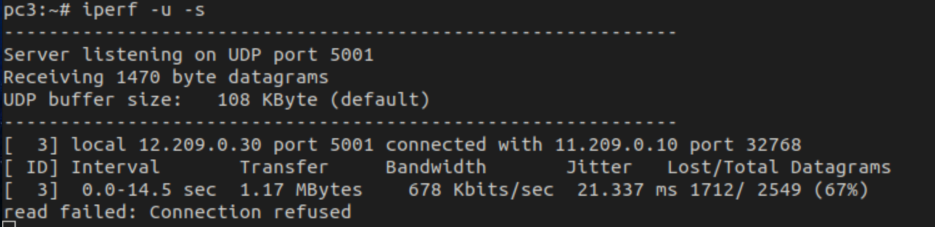
\includegraphics[width=0.8\textwidth]{ej1.3.3_3_a}
		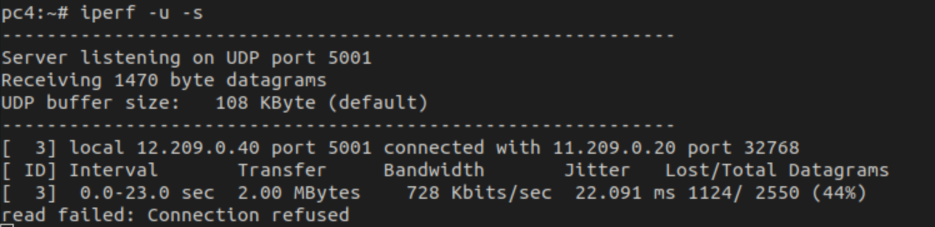
\includegraphics[width=0.8\textwidth]{ej1.3.3_3_b}
	\end{figure}
	\item Carga la captura en wireshark y muestra cada uno de los flujos de forma gráfica. Incluye una
	imagen en la memoria que muestre los flujos de forma gráfica. Explica la evolución en el tiempo
	del ancho de banda medido para cada uno de los flujos.
	\begin{figure}[H]
		\centering
		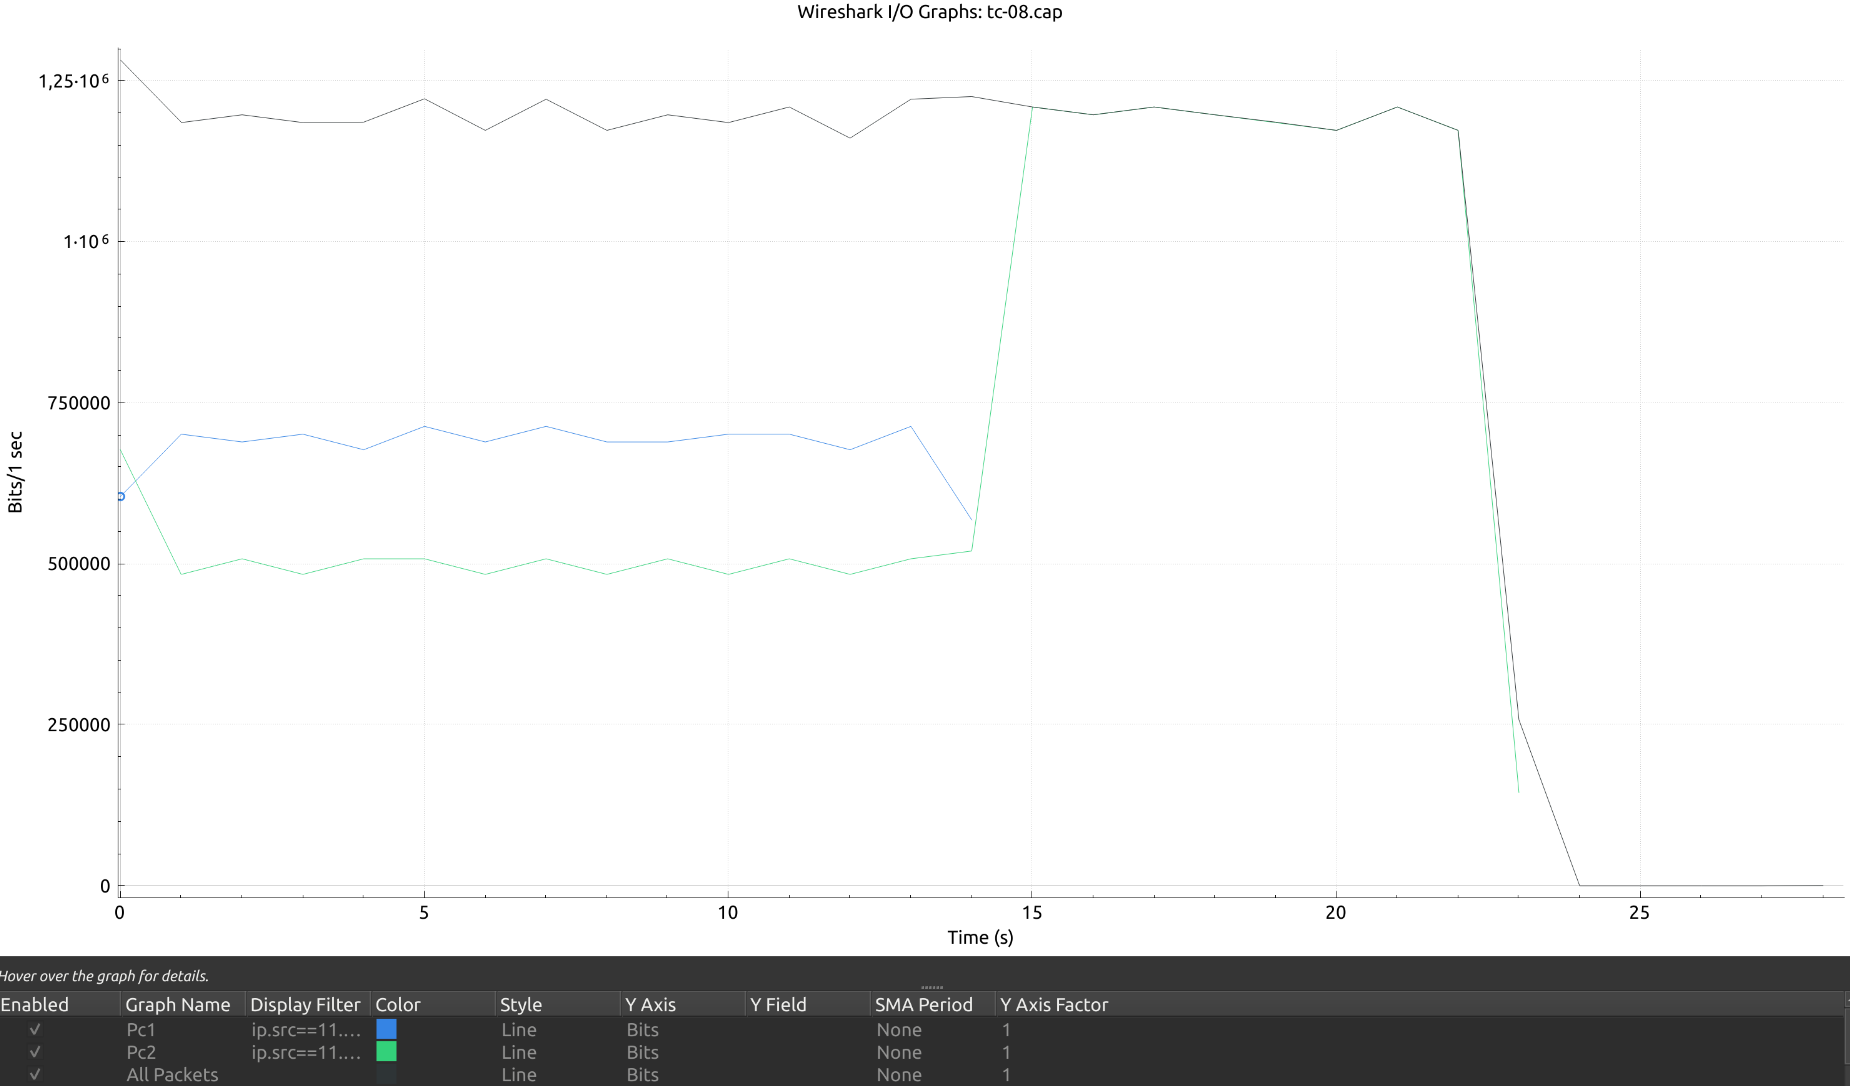
\includegraphics[width=0.8\textwidth]{ej1.3.3_4}
	\end{figure}
	Durante la parte que esta el flujo de pc1 es igual que en la captura anterior. La diferencia entre ambas es en la parte donde solo esta pc2, ya que en esta, en vez de estar limitada a 0.5 mbit/s, aquí usa todo el ancho de banda disponible.
\end{enumerate}

\chapter{Diffserv}
Descarga tu escenario de red para esta práctica del siguiente enlace:

\begin{center}
	https://mobiquo.gsyc.urjc.es/practicas/ror/p4.html
\end{center}

Descomprime el fichero que contiene el escenario de NetGUI lab-DiffServ.tgz para realizar la práctica de diffServ en Linux.\\

\begin{figure}[h]
	\centering
	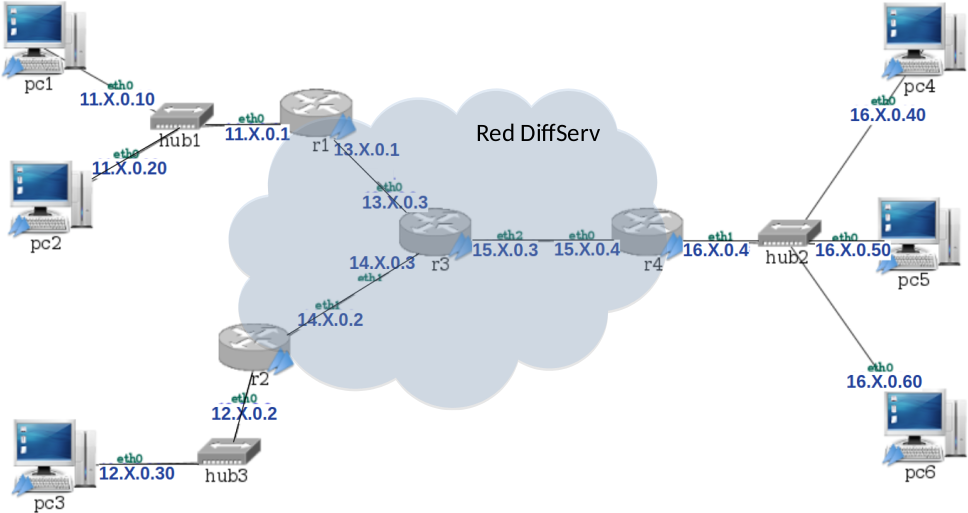
\includegraphics[width=0.8\textwidth]{enunciado2}
	\caption{Escenario para DiffServ}
\end{figure}

En el escenario de la figura 2 se va a configurar la red para que el tráfico desde pc1, pc2 y pc3
envíen paquetes a pc4, pc5 y pc6 atravesando una red diffServ. Configura las direcciones IP en tu
escenario utilizando las tus 4 subredes de la práctica 1, y elige las subredes que quieras como subdred
13.X.0.0/24 y subdred 14.X.0.0/24.\\

Para esta práctica se distinguirán 4 calidades diferentes, con los códigos EF, AF31, AF21 y AF11.
\section{Configuración de función policing y marcado de tráfico en DSCP}
Utiliza la herramienta tc para garantizar que el tráfico que entra en r1 cumple las siguientes
características:
\begin{itemize}
	\item La red diffServ deberá garantizar a la entrada los siguientes anchos de banda para pc1, descartando el tráfico sobrante:
	\begin{itemize}
		\item Flujo 1: máximo 1.2mbit con ráfaga 10k para el tráfico dirigido a pc4, marcado con calidad
		EF. Si se supera este ancho de banda, el tráfico quedará clasificado dentro del flujo 2.
		\item Flujo 2: máximo de 600kbit y ráfaga 10k, marcado con calidad AF31. Si se supera este
		ancho de banda, el tráfico será descartado definitivamente en r1.
	\end{itemize}
	\item La red diffServ deberá garantizar a la entrada los siguientes anchos de banda para pc2, descartando el tráfico sobrante:
	\begin{itemize}
		\item Flujo 3: máximo 300kbit con ráfaga 10k para el tráfico dirigido a pc5, marcado con AF21.
		Si se supera este ancho de banda, el tráfico quedará clasificado dentro del flujo 4.
		\item Flujo 4: máximo de 400kbit y ráfaga 10k, marcado con AF11. Si se supera este ancho de
		banda, el tráfico será descartado definitivamente en r1.
	\end{itemize}
\end{itemize}
Utiliza la herramienta tc para garantizar que el tráfico que entra en r2 cumple las siguientes
características:
\begin{itemize}
	\item La red diffServ deberá garantizar a la entrada los siguientes anchos de banda para pc3, descartando el tráfico sobrante:
	\begin{itemize}
		\item Flujo 5: máximo 400kbit con ráfaga 10k dirigido a pc6, marcado con AF31. Si se supera
		este ancho de banda, el tráfico quedará clasificado dentro del flujo 6.
		\item Flujo 6: máximo 300kbit con ráfaga 10k dirigido a pc6, marcado con AF21. Si se supera
		este ancho de banda, el tráfico quedará clasificado dentro del flujo 7.
		\item Flujo 7: máximo 100kbit con ráfaga 10k, marcado con AF11. Si se supera este ancho de
		banda, el tráfico será descartado definitivamente en r2.
	\end{itemize}
\end{itemize}
\begin{enumerate}
	\item Realiza scripts para r1 y otro para r2 donde se configuren estos perfiles de tráfico. Incluye dichos
	scripts en la memoria.\\
	
	 Ver \ref{script-r1} para r1 y \ref{script-r2} para r2.
	\item Inicia capturas: \textcolor{blue}{diffServ-01.cap} en la subdred 13.X.0.0/24, \textcolor{blue}{diffServ-02.cap} en la subdred
	14.X.0.0/24 y \textcolor{blue}{diffServ-03.cap} en la subdred 15.X.0.0/24 para que capture el tráfico que se
	genera en tu escenario por el envío ”simultáneo” de:
	\begin{itemize}
		\item Desde el pc1 2M a pc4
		\item Desde el pc2 1.5M a pc5
		\item Desde el pc3 1M a pc6
	\end{itemize}
	\item Interrumpe las capturas, al menos 1 minuto después de que la transmisión haya terminado.
	Comprueba que el resultado es el esperado:
	\begin{itemize}
		\item El tráfico que entra en la red diffServ es el que se ha especificado en el control de admisión.
		\item El tráfico está marcado según las especificaciones anteriores.
	\end{itemize}
	Para ello, consulta las gráficas IO graphs de Wireshark aplicando los filtros sobre las marcas
	DSCP de tal forma que se muestre cada calidad marcada de cada una de las fuentes:
	\begin{itemize}
		\item Tráfico de EF
		\item Tráfico de AF31
		\begin{itemize}
			\item Total
			\item Con origen en pc1.
			\item Con origen en pc3.
		\end{itemize}
		\item Tráfico de AF21
		\begin{itemize}
			\item Total
			\item Con origen en pc2.
			\item Con origen en pc3.
		\end{itemize}
		\item Tráfico de AF11
		\begin{itemize}
			\item Total
			\item Con origen en pc2.
			\item Con origen en pc3.
		\end{itemize}
	\end{itemize}
	Explica los resultados obtenidos e incluye todas las gráficas que consideres necesarias en la
	memoria.\\
	
	Las 2 gráficas importantes son las dos primeras, ya que la tercera es la suma de estas dos.\\
	
	Luego, en la primera captura se puede ver como pc1 ocupa al máximo los flujos que tiene disponibles y se descarta los 0.2 mbit/s sobrantes. Y con el flujo desde pc2 ocurre los mismo, ya que este ocupa los dos flujos que tiene disponible (el de AF21 y 11) en su totalidad, descartando 0.8 mbit/s de datos.
	\begin{figure}[H]
		\centering
		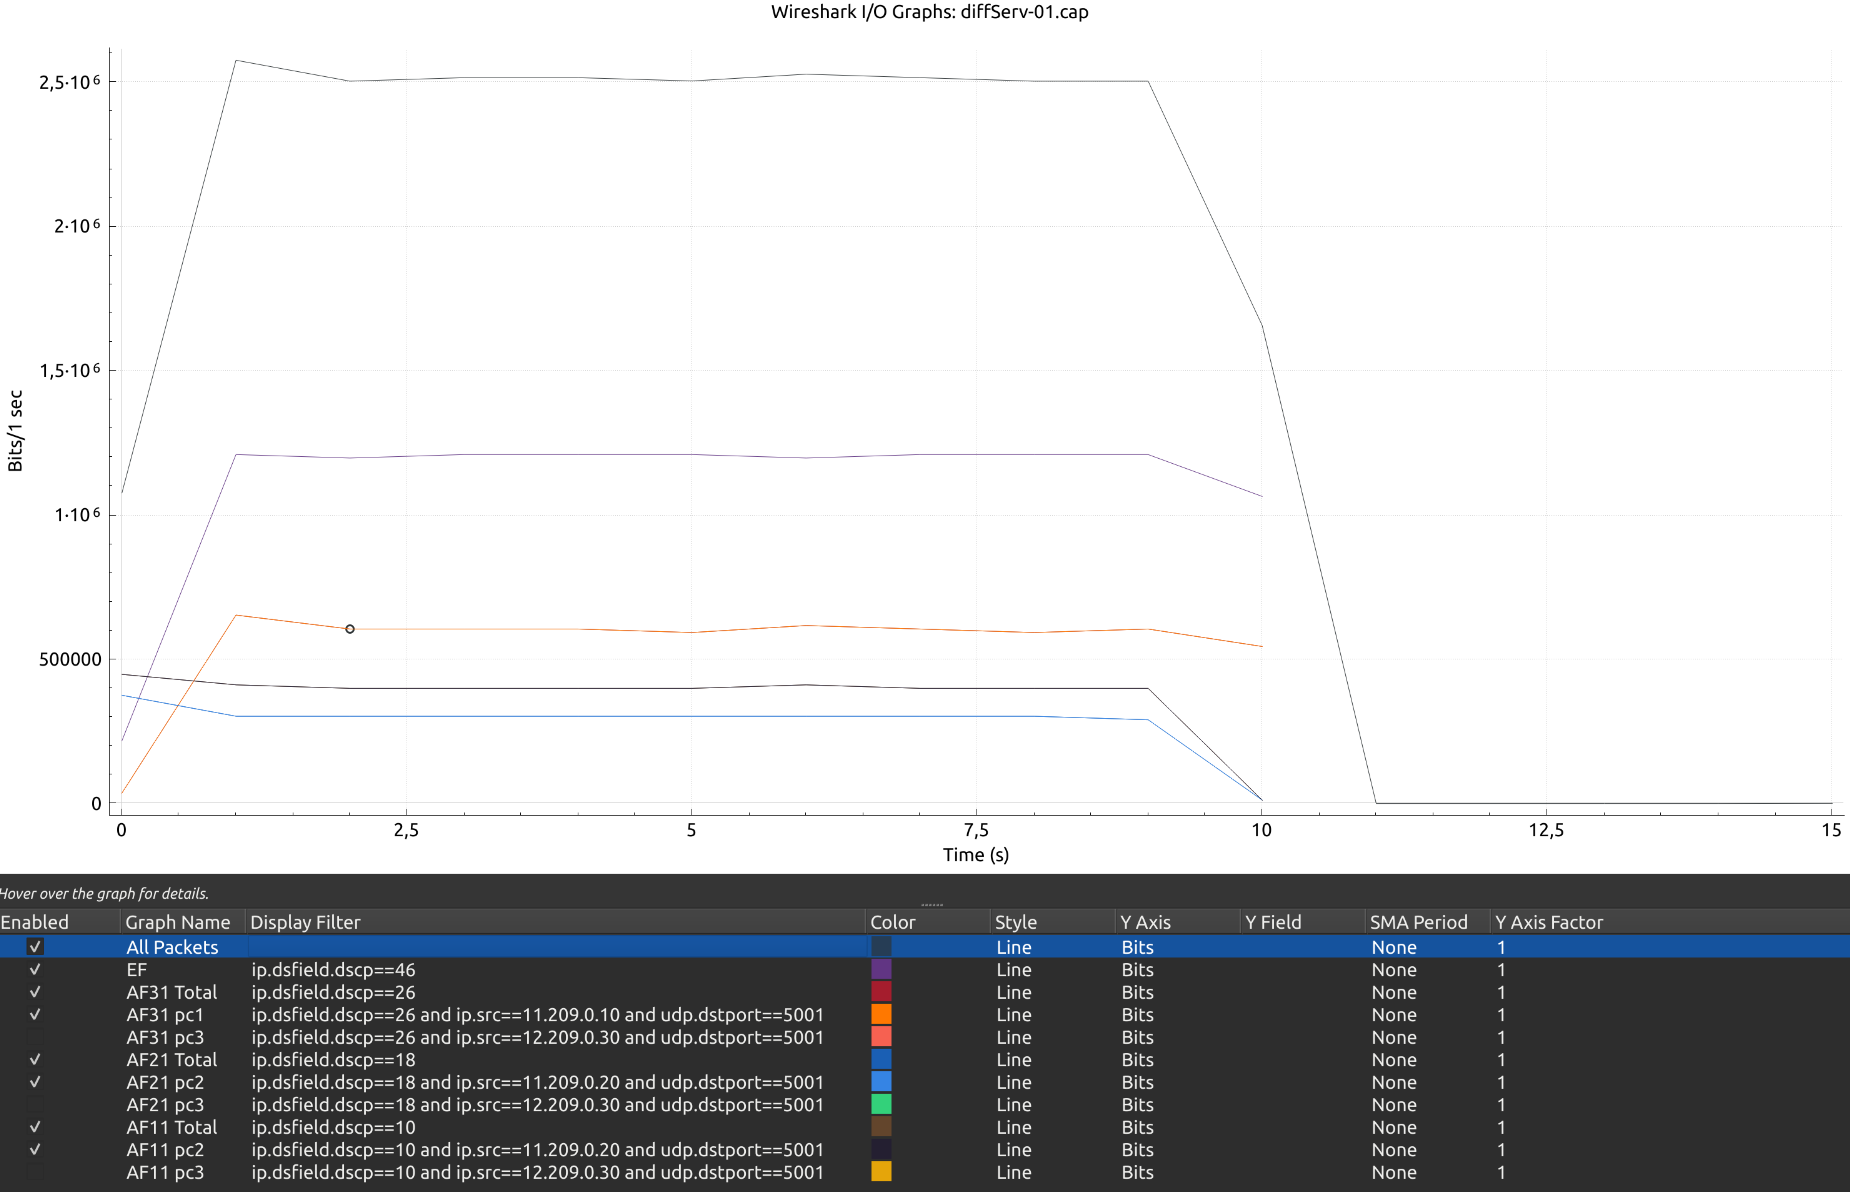
\includegraphics[width=0.8\textwidth]{ej2.1_3_13}
	\end{figure}
	En la segunda captura solo se ven los flujos que utiliza pc3, que son AF31, 21 y 11, y los utiliza también en su totalidad, por lo que el resto de datos, 0.2 mbit/s, se descartan.
	\begin{figure}[H]
		\centering
		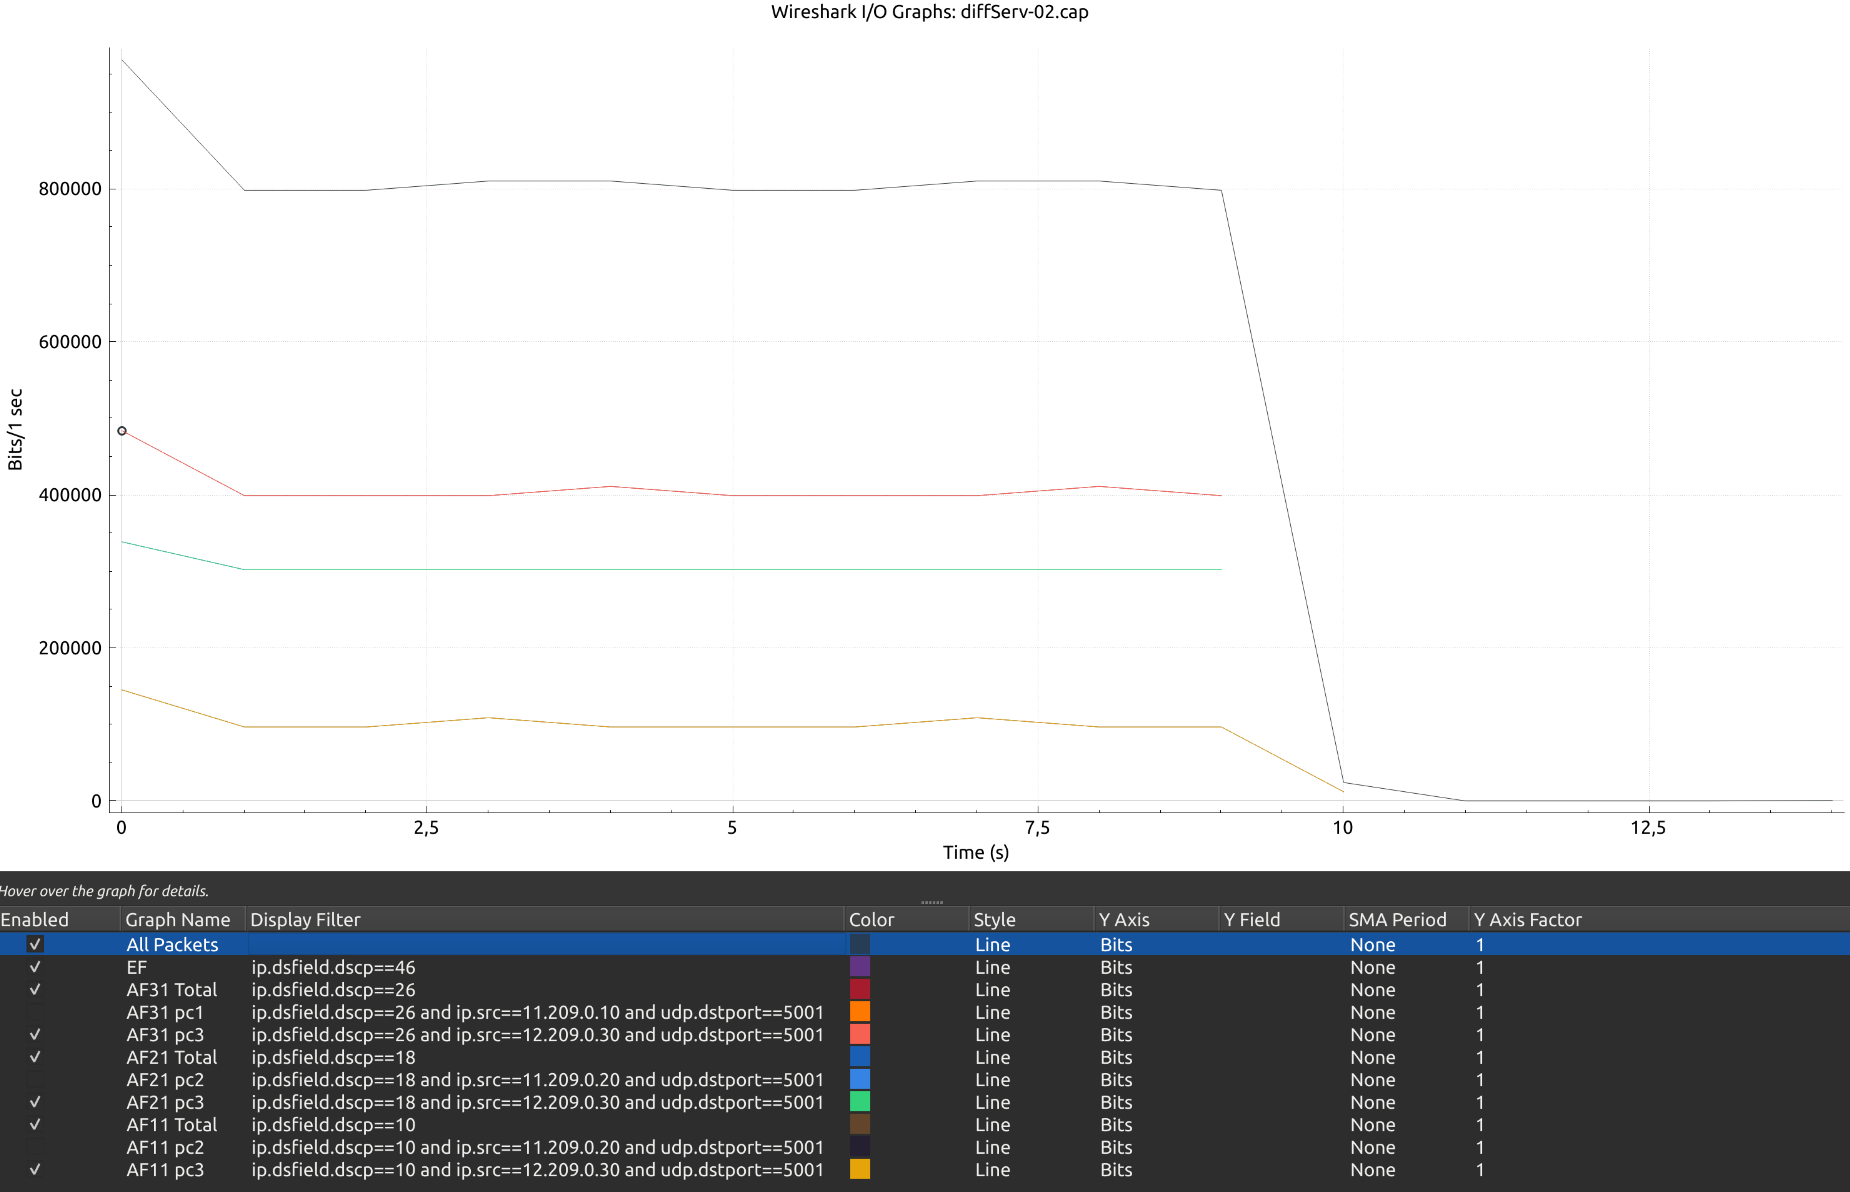
\includegraphics[width=0.8\textwidth]{ej2.1_3_14}\\
		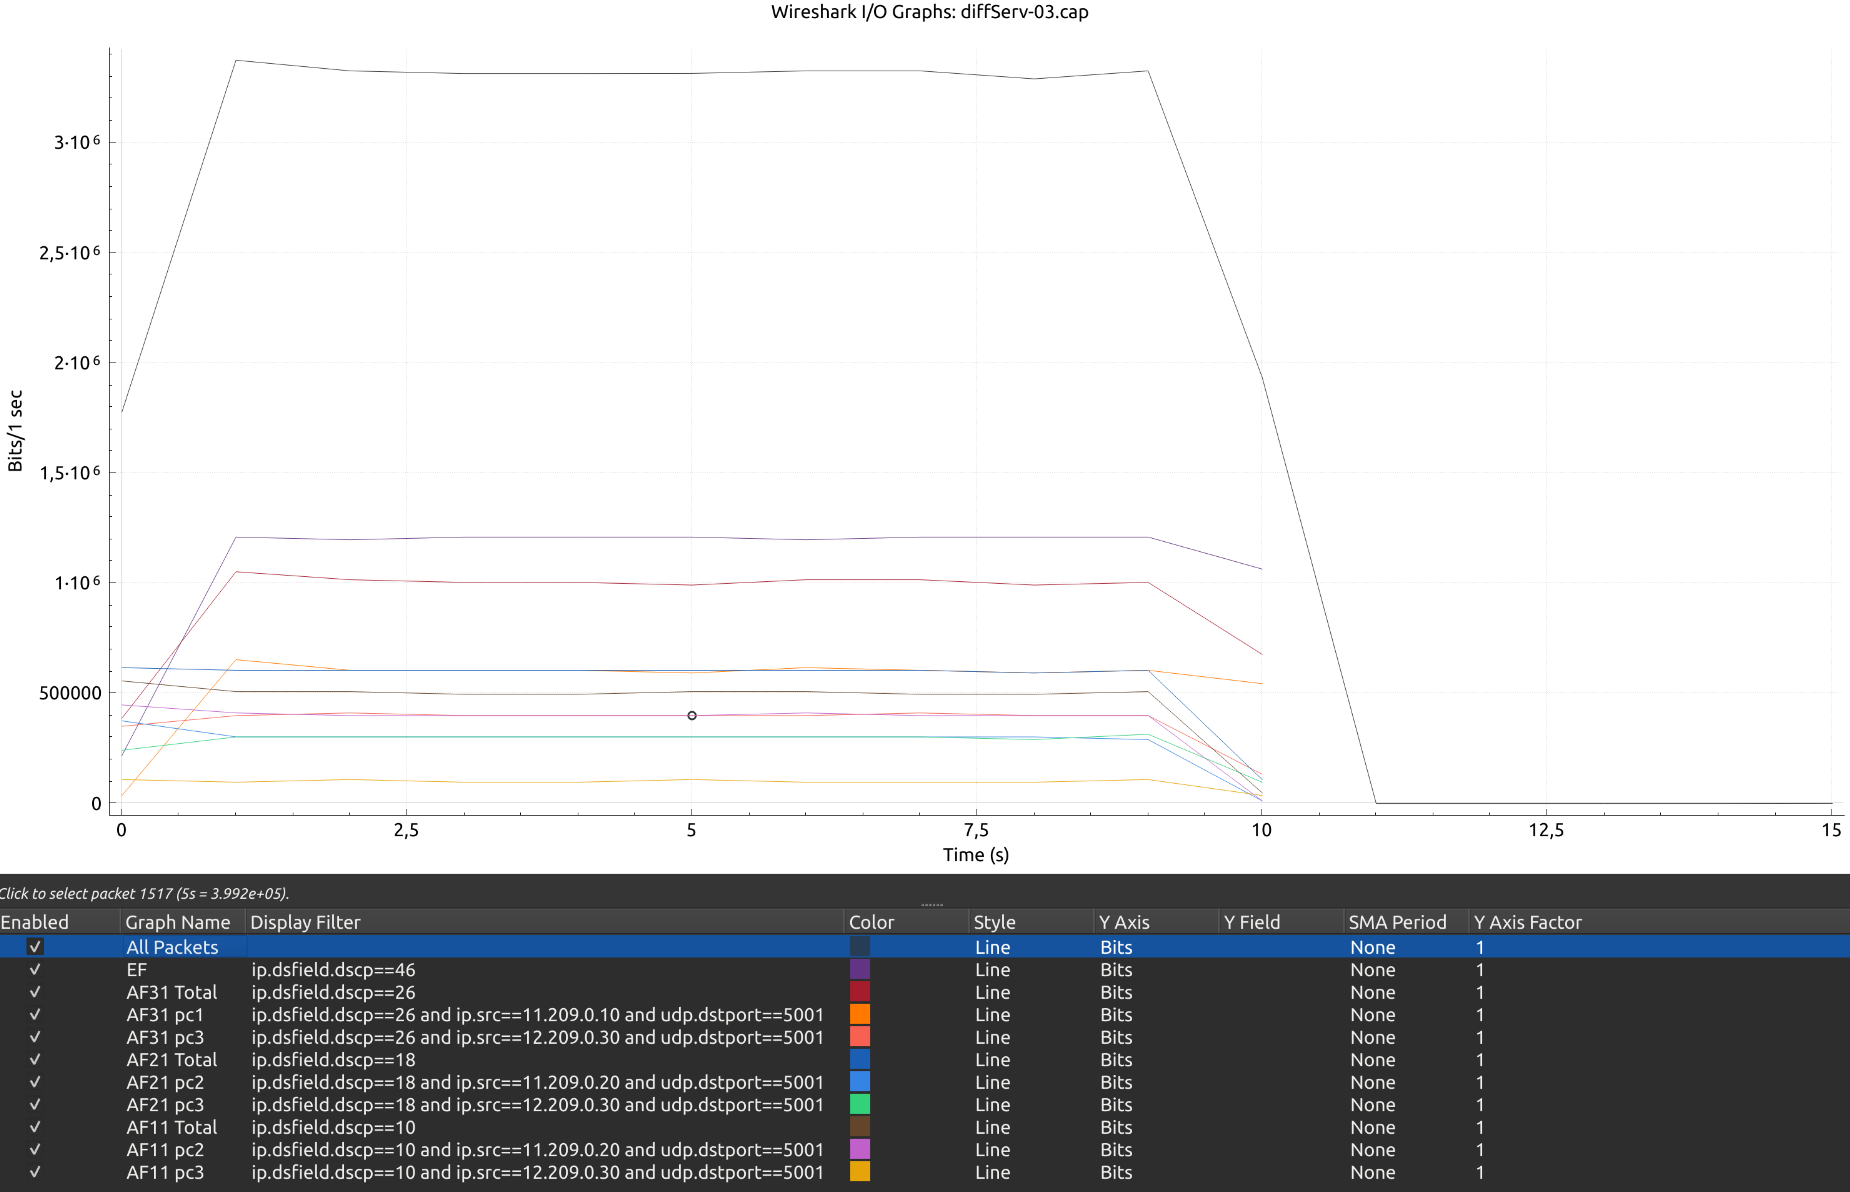
\includegraphics[width=0.8\textwidth]{ej2.1_3_15}
	\end{figure}
\end{enumerate}
\section{Tratamiento de tráfico en función del marcado DSCP}
Mantén la configuración realizada en r1, r2.\\

Se establecen los siguientes parámetros de calidad dentro del router del núcleo diffServ (r3) para
cada una de las calidades definidas. Configura HTB con ancho de banda 2.4Mbit para compartir entre
todos los flujos con el siguiente patrón:
\begin{itemize}
	\item EF: HTB 1Mbit como mínimo y 1Mbit como máximo.
	\item AF31: HTB 500kbit como mínimo y 500kbit como máximo.
	\item AF21: HTB 400kbit como mínimo y 400kbit como máximo.
	\item AF11: HTB 200kbit como mínimo y 200kbit como máximo.
\end{itemize}
\begin{enumerate}
	\item Realiza un script para r3 donde se configure esta disciplina de cola según el marcado de los
	paquetes e incluye dicho script en la memoria.\\
	
	Ver \ref{script-r3}.
	\item Inicia una captura (\textcolor{blue}{diffServ-04.cap}) en la subdred 15.X.0.0/24 para que capture el tráfico que
	se genera en tu escenario por el envío ”simultáneo” de:
	\begin{itemize}
		\item Desde pc1: 2M a pc4
		\item Desde pc2: 1.5M a pc5
		\item Desde pc3: 1M a pc6
	\end{itemize}
	Espera al menos 2 minutos después de que haya terminado de enviarse el tráfico de pc1, pc2 y
	pc3 antes de interrumpir la captura de tráfico.
	\item Comprueba que el resultado es el esperado, es decir, el tráfico sigue el perfil indicado en las
	especificaciones anteriores. Para ello, consulta las gráficas IO graphs de Wireshark aplicando
	los filtros sobre las marcas DSCP de tal forma que se muestre cada calidad marcada de cada
	una de las fuentes incluyendo dichas imágenes en la memoria:
	\begin{itemize}
		\item Tráfico de EF
		\item Tráfico de AF31
		\item Tráfico de AF21
		\item Tráfico de AF11
	\end{itemize}
	Explica los resultados obtenidos y explica si alguno de los flujos ha encolado tráfico para enviarlo
	posteriormente a los 10 segundos que dura la transmisión de iperf.\\
	
	Es bastante fácil de ver que todos los flujos encolan tráfico para su posterior reenvío, ya que envían mensajes pasados los 10 segundos que dura la transmisión. Esto también se puede ver al comparar numéricamente el flujo que entraba en la última captura del apartado anterior con en nuevo filtro de salida.
	\begin{figure}[H]
		\centering
		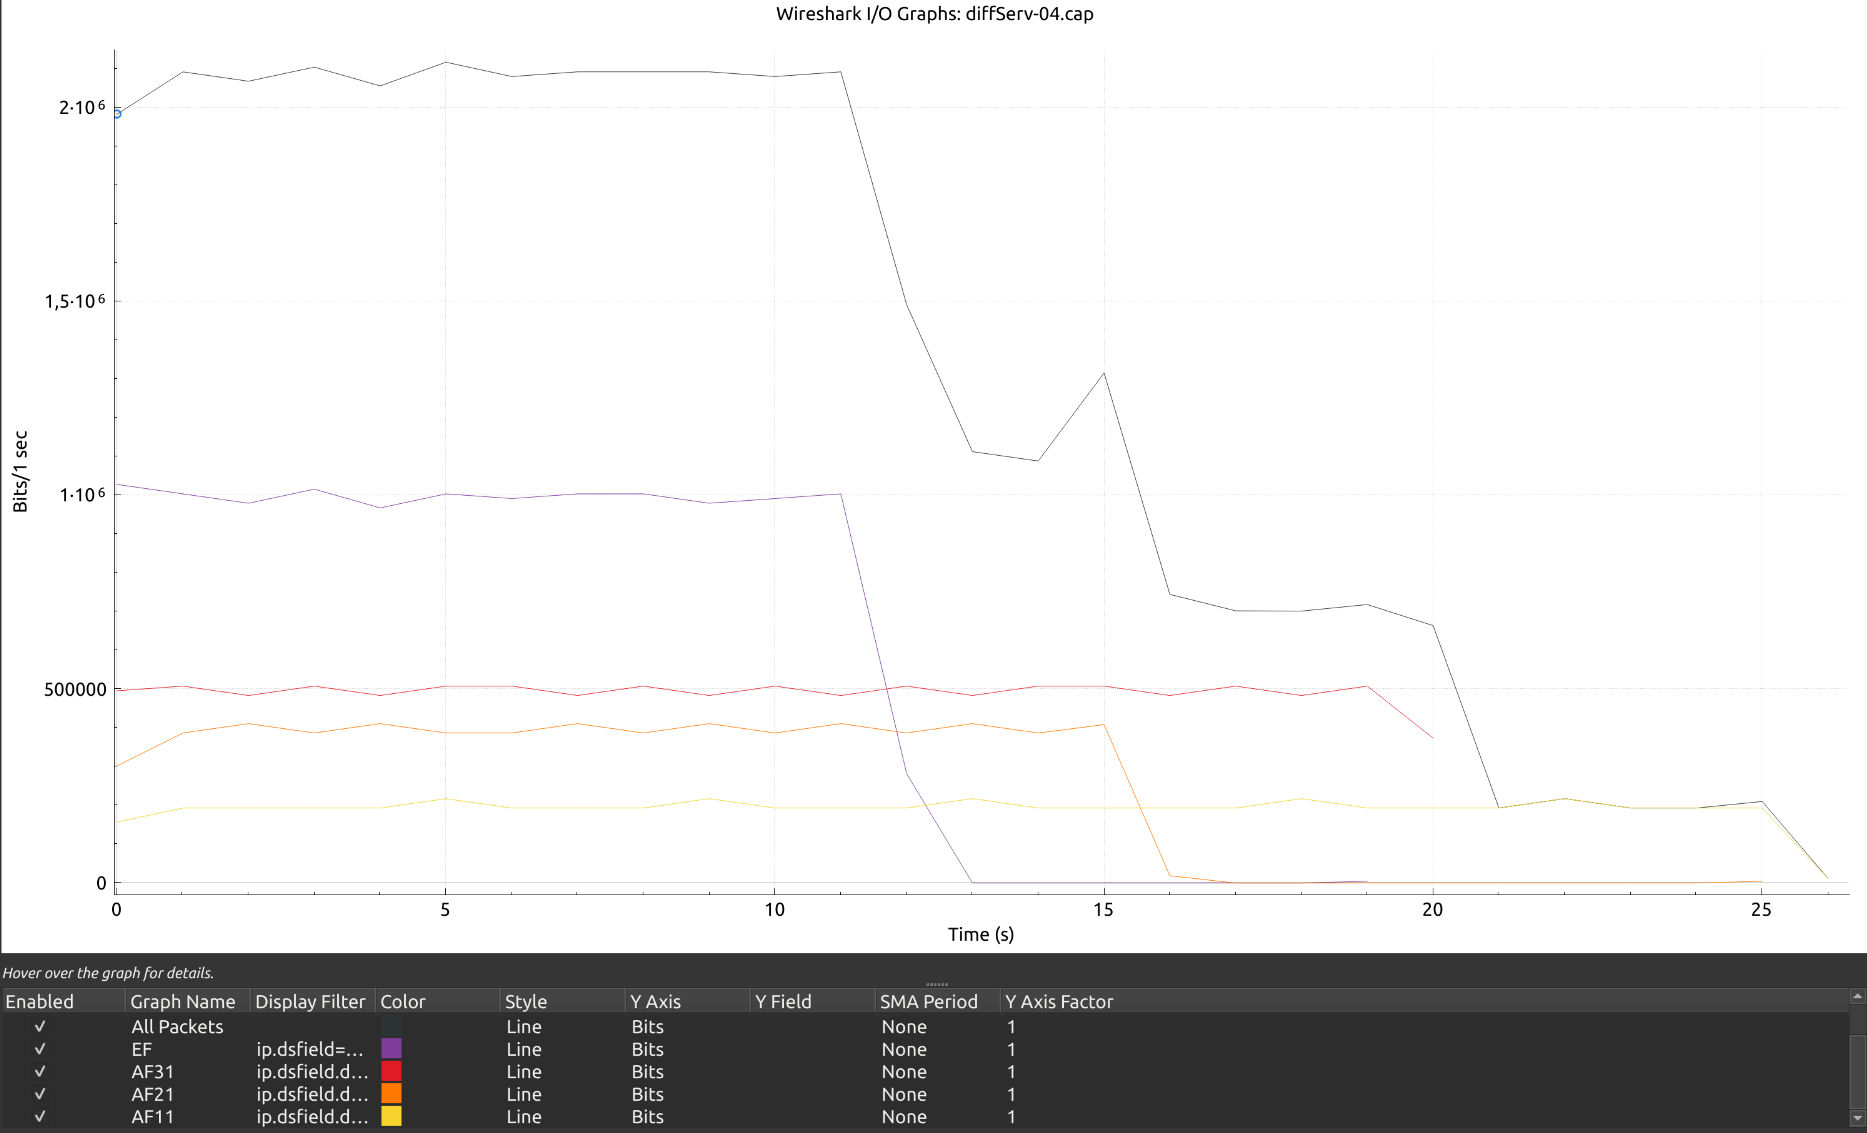
\includegraphics[width=0.8\textwidth]{ej2.2_3}
	\end{figure}
	\item Modifica la configuración de HTB en r3 para que si algún flujo no está utilizando el ancho de
	banda que tiene garantizado lo puedan usar el resto de flujos y vuelve a hacer una captura de
	tráfico (\textcolor{blue}{diffServ-05.cap}) en la subdred 15.X.0.0/24. Explica qué modificaciones has tenido
	que hacer en el script.\\
	
	Las modificaciones han sido cambiar el ceil de los flujos por el ceil máximo. Ver \ref{script-r3}.
	\item Explica los resultados obtenidos e incluye las gráficas IO graphs que consideres necesarias.\\
	
	En esta captura se puede ver como el flujo de datos totales se mantiene constante en el flujo máximo de 2.4 mbit/s y que ya no es necesario encolar todo el tráfico.\\
	
	El procedente de EF no se encola ya que tiene mayor prioridad, y ahora reenvía datos a 1.2 mbit/s en vez de a 1 como anteriormente.
	
	Con el resto de flujos ocurre algo similar pero siguen encolando el tráfico, y también se ve que cuando acaba un flujo con mayor prioridad estos sufren un aumento en el ancho de banda.\\
	
	Y por último el tiempo total se ve reducido en 10 segundos respecto a los 25 del apartado anterior, al usar de manera más eficiente el flujo total.
	\begin{figure}[H]
		\centering
		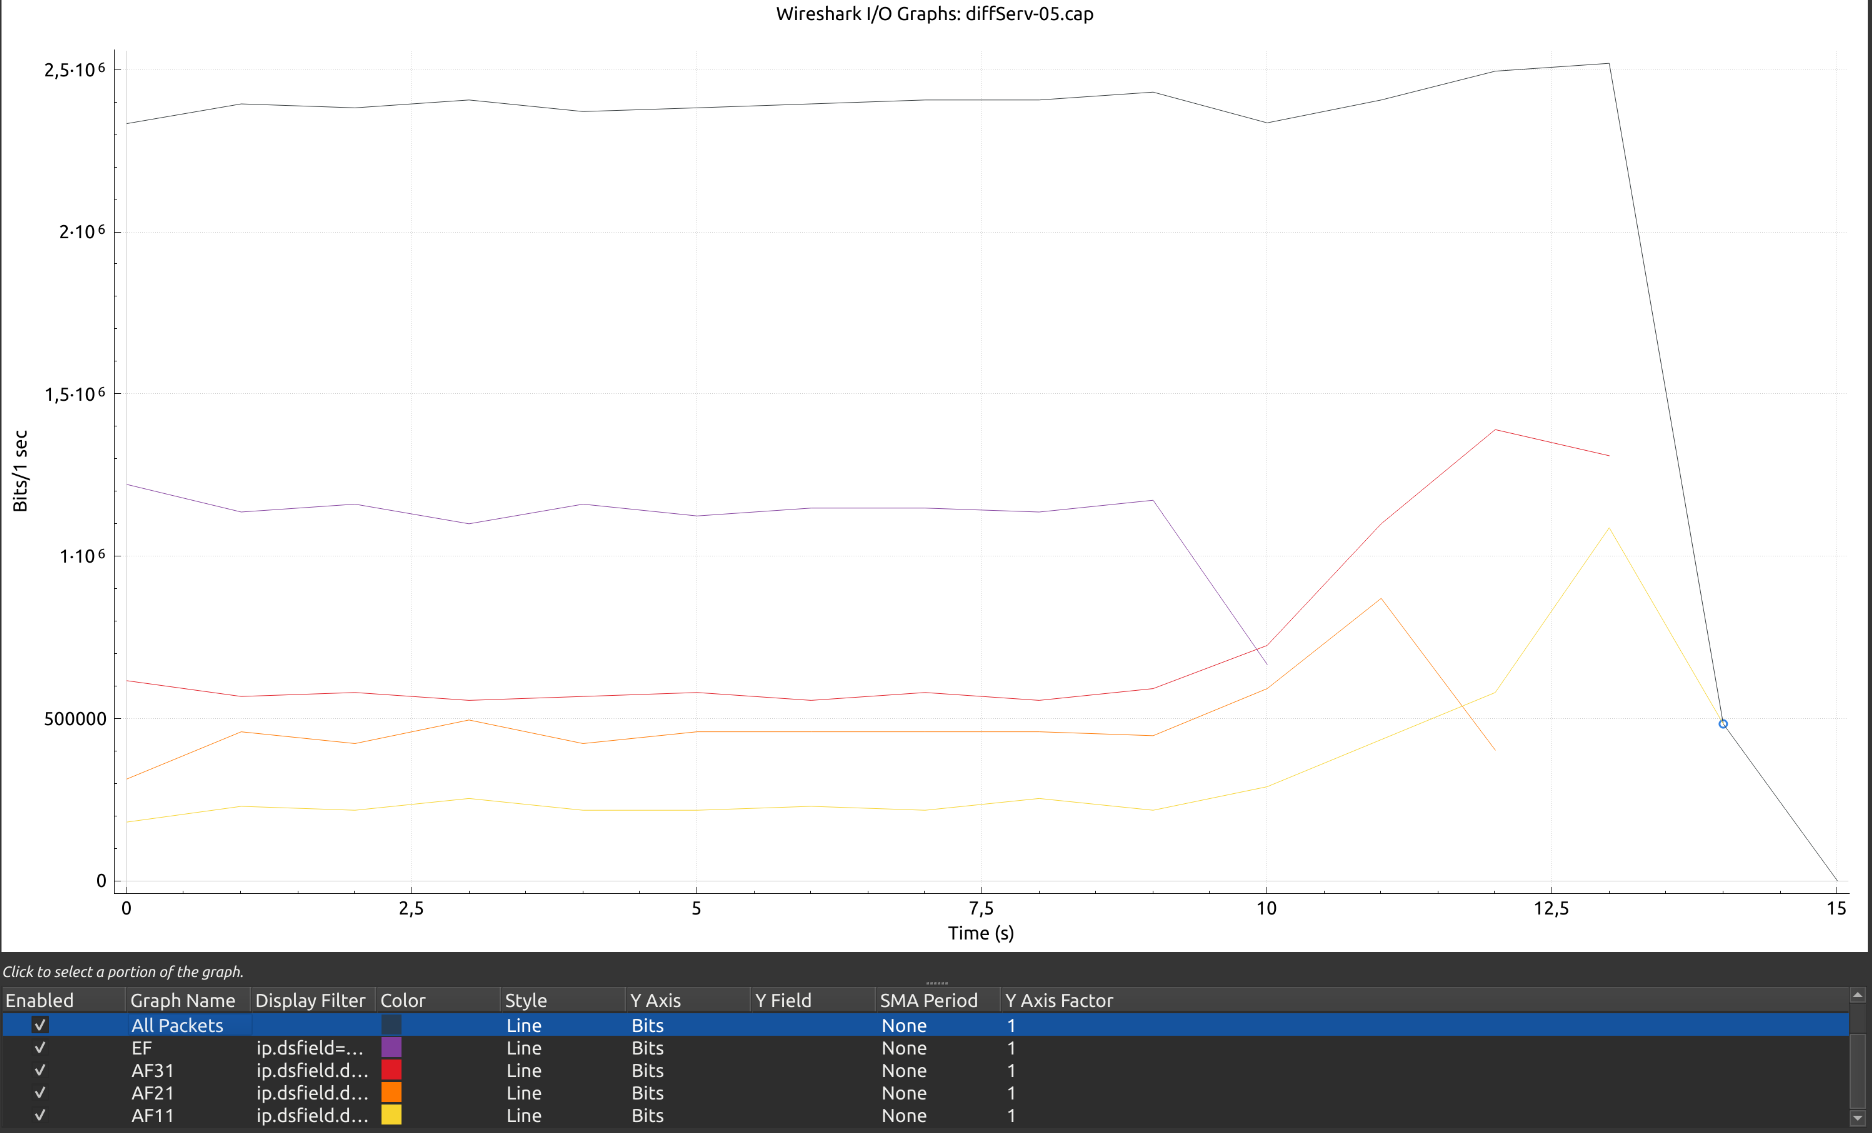
\includegraphics[width=0.8\textwidth]{ej2.2_5}
	\end{figure}
\end{enumerate}
\chapter{Scripts}
\lstinputlisting[caption=tc-ingress.sh,language=Bash,basicstyle=\tiny,label=tc-ingress]{include/tc-ingress.sh}
\lstinputlisting[caption=tc-egress-tbh.sh,language=Bash,basicstyle=\tiny,label=tc-egress-tbh]{include/tc-egress-tbh.sh}
\lstinputlisting[caption=tc-egress-tbh-prio.sh,language=Bash,basicstyle=\tiny,label=tc-egress-tbh-prio]{include/tc-egress-tbh-prio.sh}
\lstinputlisting[caption=tc-egress-htb.sh,language=Bash,basicstyle=\tiny,label=tc-egress-htb]{include/tc-egress-htb.sh}
\lstinputlisting[caption=script-r1.sh,language=Bash,basicstyle=\tiny,label=script-r1]{include/script-r1.sh}
\lstinputlisting[caption=script-r2.sh,language=Bash,basicstyle=\tiny,label=script-r2]{include/script-r2.sh}
\lstinputlisting[caption=script-r3.sh,language=Bash,basicstyle=\tiny,label=script-r3]{include/script-r3.sh}
\end{document}
